%%%%%%%%%%%%%%%%%%%%%%%%%%%%%%%%%%%%%%%%%%%%%%%%%%%%%%%%
%   |------------------------------------------|       %
%   | Web App embebida en dispositivos móviles |       %
%   |  para la gestión de registros sobre la   |       %
%   |   contaminación de afluentes y ríos.     |       %
%   |                                          |       %
%   |          Proyecto de graduación          |       %
%   |__________________________________________|       %
%                                                      %
%   Autores                                            %
%   -------                                            %
%                                                      %
% * Bruno, Ricardo Hugo (CX 1409686)                   %
%     rburnount@gmail.com                              %
% * Gomez Veliz, Kevin Shionen (CX 1411828)            %
%     ing.gomezvelizkevin@gmail.com                    %
%                                                      %
%   Tutor                                              %
%   -------                                            %
%                                                      %
% * Ing. Cohen, Daniel Eduardo                         %
%        dcohen.tuc@gmail.com                          %
%                                                      %
%   Cotutor                                            %
%   -------                                            %
%                                                      %
% * Ing. Nieto, Luis Eduardo                           %
%        lnieto@herrera.unt.edu.ar                     %
%                                                      %
%                                                      %
%%%%%%%%%%%%%%%%%%%%%%%%%%%%%%%%%%%%%%%%%%%%%%%%%%%%%%%%

\chapter{Disciplina de Diseño}
	\label{chap:disenio}
	Por el Principio de Pareto\footnote{Cuando se habla de los costes de desarrollo de software enunciarse de la siguiente manera: ``El 80\% del esfuerzo de desarrollo (en tiempo y recursos) produce el 20\% del código, mientras que el 80\% restante es producido con tan sólo un 20\% del esfuerzo''}, se hicieron los diagramas relevantes. Como se procura tener homogeneidad en la implementación de las clases, basta un solo diagrama de cada tipo para una clase, para describir también el comportamiento de las otras clases.

	\section{Descripción Textual de Casos de Uso}
		%#############################################################################
		%#   
		%#   Caso de uso 1
		%#
		%#############################################################################
		\subsection{Caso de Uso 01: Un usuario no registrado desea registrarse en el sistema.}
			\begin{longtable}{|l|p{5.5cm}|l|p{2cm}|l|p{1.9cm}|} \hline
					\cellcolor{grisOscuro} CU01 & \multicolumn{4}{|l|}{  \cellcolor{grisOscuro} Registrar} &  \cellcolor{grisClaro}\multirow{2}{1cm}{} \\ \cline{1-5}
					\cellcolor{grisOscuro} Revisa: &  \cellcolor{grisClaro} &  \cellcolor{grisOscuro} Fecha &  \cellcolor{grisClaro} &  \cellcolor{grisOscuro} Firma: & \cellcolor{grisClaro} \\ \hline
					\multicolumn{6}{|p{15cm}|}{ \textbf{Resumen: } Este caso de uso permite a los usuarios registrarse como usuarios de la aplicación, permitiendo introducir sus datos personales

					} \\ \hline

					\multicolumn{6}{|p{15cm}|}{ \textbf{Actores: } Usuario (primario). Servidor (en adelante S. Secundario)

					} \\ \hline

					\multicolumn{6}{|p{15cm}|}{ \textbf{Personal Involucrado y Metas: }
					
					\emph{Usuario:} quiere transformarse en un usuario del sistema, así pueda realizar las transacciones con la aplicación de un modo seguro y personalizado.
					
					\emph{Servidor: } quiere registrar la mayor cantidad de usuarios posibles y que el proceso sea lo más rápido y seguro posible.
					} \\ \hline

					\multicolumn{6}{|p{15cm}|}{ \textbf{Precondiciones: } El usuario no está registrado en la aplicación

					} \\ \hline

					\multicolumn{6}{|p{15cm}|}{ \textbf{Poscondiciones: } Se registra al usuario como usuario de la aplicación. El usuario puede realizar operaciones en la aplicación.

					} \\ \hline

					\multicolumn{6}{|p{15cm}|}{ \textbf{Escenario Principal: }
							\begin{enumerate}
									\item El usuario ejecuta la aplicación móvil (en adelante APP) en su Smartphone y decide registrarse.
									\item APP muestra un formulario de carga donde ingresa sus datos personales y su nombre de usuario y contraseña.
									\item APP verifica los datos ingresados.
									\item APP solicita a S el registro del usuario.
									\item S registra al usuario y lo informa a APP.
									\item APP da la bienvenida al usuario.
							\end{enumerate}

					} \\ \hline

					\multicolumn{6}{|p{15cm}|}{ \textbf{Flujos Alternativos: }

					\textbf{A1: El sistema encuentra algún fallo para comunicarse con S}

					La secuencia A1 comienza en el punto 4 del escenario principal.
					\begin{enumerate}
							\setcounter{enumi}{4}
							\item APP informa al usuario el problema de conexión a través de un mensaje por la pantalla.
					\end{enumerate}

					El escenario vuelve al punto 4.

					\textbf{A2: Nombre de usuario existente}
					
					La secuencia A2 comienza en el punto 4 del escenario principal.
					\begin{enumerate}
							\setcounter{enumi}{4}
							\item S comunica que el nombre de usuario es existente.
					\end{enumerate}

					El escenario vuelve al punto 3.

					\textbf{A3: Contraseña inválida o no coincide con la confirmación}
					
					La secuencia A3 comienza en el punto 3 del escenario principal.
					\begin{enumerate}
							\setcounter{enumi}{3}
							\item APP informa el problema a través de un mensaje por pantalla.
					\end{enumerate}

					El escenario vuelve al punto 2.

					\textbf{A4: Dirección de correo electrónico existente}
					
					La secuencia A4 comienza en el punto 4 del escenario principal.
					\begin{enumerate}
							\setcounter{enumi}{4}
							\item S comunica que la dirección de correo electrónico es existente.
					\end{enumerate}

					El escenario vuelve al punto 2.

					\textbf{A5: Tipo de datos ingresados de manera incorrecta}
					
					La secuencia A5 comienza en el punto 3 del escenario principal.
					\begin{enumerate}
							\setcounter{enumi}{3}
							\item APP informa el problema a través de un mensaje por pantalla.
					\end{enumerate}

					El escenario vuelve al punto 2.

					} \\ \hline

					\multicolumn{6}{|p{15cm}|}{ \textbf{Requisitos de Interfaz de Usuario para todos los casos de uso: }

					Smartphone con SO Android o iOS o Windows Mobile, con pantalla táctil, cámara y GPS integrado.
					
					} \\ \hline

					\multicolumn{6}{|p{15cm}|}{ \textbf{Requisitos No-Funcionales para todos los casos de uso: }

					\emph{Tiempo de respuesta:} la interfaz debe responder dentro de un tiempo máximo de 3 segundos en una velocidad efectiva de conexión con el servidor a través de 3G.

					\emph{Disponibilidad:} debe poder accederse a toda hora, los 365 días del año.

					} \\ \hline

			\end{longtable}



		%#############################################################################
		%#   
		%#   Caso de uso 2
		%#
		%#############################################################################
		\subsection{Caso de Uso 02: Un usuario registrado desea iniciar sesión en la aplicación movil.}
			\begin{longtable}{|l|p{5.5cm}|l|p{2cm}|l|p{1.9cm}|} \hline
				\cellcolor{grisOscuro} CU02 & \multicolumn{4}{|l|}{  \cellcolor{grisOscuro} Iniciar Sesión} &  \cellcolor{grisClaro}\multirow{2}{1cm}{} \\ \cline{1-5}
				\cellcolor{grisOscuro} Revisa: &  \cellcolor{grisClaro} &  \cellcolor{grisOscuro} Fecha &  \cellcolor{grisClaro} &  \cellcolor{grisOscuro} Firma: & \cellcolor{grisClaro} \\ \hline
				\multicolumn{6}{|p{15cm}|}{ \textbf{Resumen: } Este caso de uso permite a los usuarios iniciar sesión con el nombre de usuario y contraseña de manera que el sistema le permita realizar tareas.

				} \\ \hline

				\multicolumn{6}{|p{15cm}|}{ \textbf{Actores: } Usuario (Primario). Servidor (en adelante S. Secundario)

				} \\ \hline

				\multicolumn{6}{|p{15cm}|}{ \textbf{Personal Involucrado y Metas: }

				\emph{Usuario:} quiere que el sistema lo reconozca como tal, así pueda realizar las tareas con la aplicación de un modo seguro y personalizado.

				\emph{App:} requiere identificar, de manera local, confiablemente a sus usuarios de manera de satisfacer sus intereses en cuando a seguridad, accesos a su cuenta personal y datos privados.

				} \\ \hline

				\multicolumn{6}{|p{15cm}|}{ \textbf{Precondiciones: } El usuario está registrado.

				} \\ \hline

				\multicolumn{6}{|p{15cm}|}{ \textbf{Poscondiciones: } Se identifica y autentica al usuario. Se conocen sus datos personales y opciones de personalización.

				} \\ \hline

				\multicolumn{6}{|p{15cm}|}{ \textbf{Escenario Principal: }

				\begin{enumerate}
					\item El usuario ejecuta la aplicación móvil (en adelante APP) en su Smartphone.
					\item APP descarga la informacion de inicio de sesión del servidor.
					\item APP solicita al usuario su nombre de usuario y contraseña.
					\item El usuario ingresa su nombre de usuario y contraseña.
					\item APP realiza el proceso de validación del usuario
					\item APP valida al usuario y comunica sus datos personales.
					\item APP da la bienvenida al usuario
				\end{enumerate}

				} \\ \hline

				\multicolumn{6}{|p{15cm}|}{ \textbf{Flujos Alternativos: }

				\textbf{A1: Nombre de usuario inexistente}
				
				La secuencia A1 comienza en el punto 4 del escenario principal.
				\begin{enumerate}
						\setcounter{enumi}{4}
						\item S comunica que el nombre de usuario es inexistente.
				\end{enumerate}

				El escenario vuelve al punto 2.

				\textbf{A2: Nombre de usuario existente pero contraseña inválida}
				
				La secuencia A2 comienza en el punto 4 del escenario principal.
				\begin{enumerate}
						\setcounter{enumi}{3}
						\item S comunica que la contraseña es inválida.
				\end{enumerate}

				El escenario vuelve al punto 2.

				} \\ \hline
			\end{longtable}

		%#############################################################################
		%#   
		%#   Caso de uso 3
		%#
		%#############################################################################
		\subsection{Caso de Uso 03: Un usuario registrado desea crear un registro}
			\begin{longtable}{|l|p{5.5cm}|l|p{2cm}|l|p{1.9cm}|} \hline
				\cellcolor{grisOscuro} CU03 & \multicolumn{4}{|l|}{  \cellcolor{grisOscuro} Crear Registro} &  \cellcolor{grisClaro}\multirow{2}{1cm}{} \\ \cline{1-5}
				\cellcolor{grisOscuro} Revisa: &  \cellcolor{grisClaro} &  \cellcolor{grisOscuro} Fecha &  \cellcolor{grisClaro} &  \cellcolor{grisOscuro} Firma: & \cellcolor{grisClaro} \\ \hline
				\multicolumn{6}{|p{15cm}|}{ \textbf{Resumen: } Este caso de uso permite al usuario crear un registro de manera que el sistema lo almacene en una base de datos para luego mostrarlo como información del mapa general

				} \\ \hline

				\multicolumn{6}{|p{15cm}|}{ \textbf{Actores: } Usuario (Primario). Servidor (en adelante S. Secundario)

				} \\ \hline

				\multicolumn{6}{|p{15cm}|}{ \textbf{Personal Involucrado y Metas: }

				\emph{Usuario:} quiere que el sistema lo reconozca como tal, así pueda realizar los registros a través de la aplicación móvil (en adelante APP) de un modo seguro y personalizado.

				\emph{Servidor:} quiere identificar confiablemente a sus usuarios de manera de satisfacer sus intereses en cuanto a seguridad y datos privados.

				} \\ \hline

				\multicolumn{6}{|p{15cm}|}{ \textbf{Precondiciones: } Los usuarios deben estar autenticados en APP

				} \\ \hline

				\multicolumn{6}{|p{15cm}|}{ \textbf{Poscondiciones: } Se almacena un nuevo registro en el sistema con los datos correspondientes necesarios para luego aportar información al mapa general

				} \\ \hline

				\multicolumn{6}{|p{15cm}|}{ \textbf{Escenario Principal: }

				\begin{enumerate}
					\item El usuario selecciona la opción para crear registro.
					\item APP solicita al usuario a través de un formulario los datos requeridos para la creacion del registro.
					\item El usuario completa el formulario y presiona un botón para finalizar.
					\item APP verifica que los tipos de datos ingresados en el formulario sean correctos y almacena el registro de forma local.
					\item APP detecta conexion a internet y envía de manera segura los datos a S para que sean validados.
					\item S valida los datos, realiza la creacion del registro y envía una confirmación.
					\item APP informa al usuario que la operación se realizó exitosamente.
				\end{enumerate}

				} \\ \hline

				\multicolumn{6}{|p{15cm}|}{ \textbf{Flujos Alternativos: }

				\textbf{A1: El sistema encuentra algún fallo para comunicarse con S}
				
				La secuencia A1 comienza en el punto 5 del escenario principal.
				\begin{enumerate}
						\setcounter{enumi}{5}
						\item APP reintenta enviar la información de manera automática por tiempo indefinido.
				\end{enumerate}

				El escenario vuelve al punto 5.

				} \\ \hline

			\end{longtable}

		%#############################################################################
		%#   
		%#   Caso de uso 4
		%#
		%#############################################################################
		\subsection{Caso de Uso 04: Un usuario registrado desea listar sus registros.}
			\begin{longtable}{|l|p{5.5cm}|l|p{2cm}|l|p{1.9cm}|} \hline
				\cellcolor{grisOscuro} CU04 & \multicolumn{4}{|l|}{  \cellcolor{grisOscuro} Listar Registros} &  \cellcolor{grisClaro}\multirow{2}{1cm}{} \\ \cline{1-5}
				\cellcolor{grisOscuro} Revisa: &  \cellcolor{grisClaro} &  \cellcolor{grisOscuro} Fecha &  \cellcolor{grisClaro} &  \cellcolor{grisOscuro} Firma: & \cellcolor{grisClaro} \\ \hline
				\multicolumn{6}{|p{15cm}|}{ \textbf{Resumen: } Este caso de uso permite a un usuario listar la información de todos los registros que realizo.

				} \\ \hline

				\multicolumn{6}{|p{15cm}|}{ \textbf{Actores: } Usuario (Primario). Servidor (Secundario).

				} \\ \hline

				\multicolumn{6}{|p{15cm}|}{ \textbf{Personal Involucrado y Metas: }

				\emph{Usuario:} quiere visualizar de manera completa la información de los registros realizados.

				\emph{Servidor:} quiere que el usuario pueda ver la información relacionada con sus registros de manera segura.

				} \\ \hline

				\multicolumn{6}{|p{15cm}|}{ \textbf{Precondiciones: } El usuario debe estar autenticado en APP.

				} \\ \hline

				\multicolumn{6}{|p{15cm}|}{ \textbf{Poscondiciones: } Se muestra un listado de registros realizados.

				} \\ \hline

				\multicolumn{6}{|p{15cm}|}{ \textbf{Escenario Principal: }

				\begin{enumerate}
					\item El usuario selecciona la opción para listar los registros realizados.
					\item APP envía la solicitud a S.
					\item S envía los datos necesarios para generar el listado de registros a APP.
					\item APP muestra el listado al usuario.
				\end{enumerate}

				} \\ \hline

				\multicolumn{6}{|p{15cm}|}{ \textbf{Flujos Alternativos: }
				
				\textbf{A1: El sistema encuentra algún fallo para comunicarse con S}
				
				La secuencia A1 comienza en el punto 2 del escenario principal.
				\begin{enumerate}
						\setcounter{enumi}{2}
						\item APP informa al usuario el problema de conexión a través de un mensaje por la pantalla.
				\end{enumerate}

				El escenario vuelve al punto 2.

				} \\ \hline

			\end{longtable}

		%#############################################################################
		%#   
		%#   Caso de uso 5
		%#
		%#############################################################################
		\subsection{Caso de Uso 05: Un usuario registrado desea ver un registro en particular}
			\begin{longtable}{|l|p{5.5cm}|l|p{2cm}|l|p{1.9cm}|} \hline
				\cellcolor{grisOscuro} CU05 & \multicolumn{4}{|l|}{  \cellcolor{grisOscuro} Ver Registro} &  \cellcolor{grisClaro}\multirow{2}{1cm}{} \\ \cline{1-5}
				\cellcolor{grisOscuro} Revisa: &  \cellcolor{grisClaro} &  \cellcolor{grisOscuro} Fecha &  \cellcolor{grisClaro} &  \cellcolor{grisOscuro} Firma: & \cellcolor{grisClaro} \\ \hline
				\multicolumn{6}{|p{15cm}|}{ \textbf{Resumen: } Este caso de uso permite al usuario ver un registro especifico que él realizo.

				} \\ \hline

				\multicolumn{6}{|p{15cm}|}{ \textbf{Actores: } Usuario (Primario). Servidor (Secundario)

				} \\ \hline

				\multicolumn{6}{|p{15cm}|}{ \textbf{Personal Involucrado y Metas: }
				
				\emph{Usuario:} quiere visualizar de manera completa la información de un registro, realizado por él, en particular.

				\emph{Servidor:} quiere que el usuario pueda ver la información relacionada con su registro de manera segura.

				} \\ \hline

				\multicolumn{6}{|p{15cm}|}{ \textbf{Precondiciones: } El usuario debe estar autenticado en APP.

				} \\ \hline

				\multicolumn{6}{|p{15cm}|}{ \textbf{Poscondiciones: } Se muestra la informacion completa de un registro.

				} \\ \hline

				\multicolumn{6}{|p{15cm}|}{ \textbf{Escenario Principal: }

				\begin{enumerate}
					\item El usuario selecciona la opción para ver un registro realizado.
					\item APP envía la solicitud a S.
					\item S envía los datos necesarios para generar la vista de un registro a APP.
					\item APP muestra el registro al usuario.
				\end{enumerate}

				} \\ \hline

				\multicolumn{6}{|p{15cm}|}{ \textbf{Flujos Alternativos: }
				
				\textbf{A1: El sistema encuentra algún fallo para comunicarse con S}
				
				La secuencia A1 comienza en el punto 2 del escenario principal.
				\begin{enumerate}
					\setcounter{enumi}{2}
					\item APP informa al usuario el problema de conexión a través de un mensaje por la pantalla.
				\end{enumerate}

				El escenario vuelve al punto 2.

				} \\ \hline
			\end{longtable}

		%#############################################################################
		%#   
		%#   Caso de uso 6
		%#
		%#############################################################################
		\subsection{Caso de Uso 06: Un usuario registrado desea ver el mapa general.}
			\begin{longtable}{|l|p{5.5cm}|l|p{2cm}|l|p{1.9cm}|} \hline
				\cellcolor{grisOscuro} CU06 & \multicolumn{4}{|l|}{  \cellcolor{grisOscuro} Ver Mapa} &  \cellcolor{grisClaro}\multirow{2}{1cm}{} \\ \cline{1-5}
				\cellcolor{grisOscuro} Revisa: &  \cellcolor{grisClaro} &  \cellcolor{grisOscuro} Fecha &  \cellcolor{grisClaro} &  \cellcolor{grisOscuro} Firma: & \cellcolor{grisClaro} \\ \hline
				\multicolumn{6}{|p{15cm}|}{ \textbf{Resumen: } Este caso de uso permite al usuario ver el mapa general con la informacion de todos los registros.

				} \\ \hline

				\multicolumn{6}{|p{15cm}|}{ \textbf{Actores: } Usuario (Primario). Servidor (Secundario)

				} \\ \hline

				\multicolumn{6}{|p{15cm}|}{ \textbf{Personal Involucrado y Metas: }
				
				\emph{Usuario:} quiere visualizar de manera completa la información del mapa general.

				\emph{Servidor:} quiere que el usuario pueda ver la información relacionada con el mapa general de forma segura.

				} \\ \hline

				\multicolumn{6}{|p{15cm}|}{ \textbf{Precondiciones: } 
				
				El usuario debe estar autenticado en APP.
				
				Debe existir al menos 1 registro en el servidor.

				} \\ \hline

				\multicolumn{6}{|p{15cm}|}{ \textbf{Poscondiciones: } Se muestra la informacion completa del mapa general.

				} \\ \hline

				\multicolumn{6}{|p{15cm}|}{ \textbf{Escenario Principal: }

				\begin{enumerate}
					\item El usuario selecciona la opción para ver el mapa general.
					\item APP envía la solicitud a S.
					\item S envía los datos necesarios para generar la vista del mapa general a APP.
					\item APP muestra el mapa general al usuario.
				\end{enumerate}

				} \\ \hline

				\multicolumn{6}{|p{15cm}|}{ \textbf{Flujos Alternativos: }
				
				\textbf{A1: El sistema encuentra algún fallo para comunicarse con S}
				
				La secuencia A1 comienza en el punto 2 del escenario principal.
				\begin{enumerate}
					\setcounter{enumi}{2}
					\item APP informa al usuario el problema de conexión a través de un mensaje por la pantalla.
				\end{enumerate}

				El escenario vuelve al punto 2.

				} \\ \hline

			\end{longtable}

		%#############################################################################
		%#   
		%#   Caso de uso 7
		%#
		%#############################################################################
		\subsection{Caso de Uso 07: Un usuario registrado desea ver su perfil.}
			\begin{longtable}{|l|p{5.5cm}|l|p{2cm}|l|p{1.9cm}|} \hline
				\cellcolor{grisOscuro} CU07 & \multicolumn{4}{|l|}{  \cellcolor{grisOscuro} Ver Perfil de Usuario} &  \cellcolor{grisClaro}\multirow{2}{1cm}{} \\ \cline{1-5}
				\cellcolor{grisOscuro} Revisa: &  \cellcolor{grisClaro} &  \cellcolor{grisOscuro} Fecha &  \cellcolor{grisClaro} &  \cellcolor{grisOscuro} Firma: & \cellcolor{grisClaro} \\ \hline
				\multicolumn{6}{|p{15cm}|}{ \textbf{Resumen: } Este caso de uso permite al usuario ver su perfil con la informacion de sus datos.

				} \\ \hline

				\multicolumn{6}{|p{15cm}|}{ \textbf{Actores: } Usuario (Primario). Servidor (Secundario)

				} \\ \hline

				\multicolumn{6}{|p{15cm}|}{ \textbf{Personal Involucrado y Metas: }
				
				\emph{Usuario:} quiere visualizar de manera completa la información de su perfil.

				\emph{Servidor:} quiere que el usuario pueda ver la información relacionada con su perfil de forma segura.

				} \\ \hline

				\multicolumn{6}{|p{15cm}|}{ \textbf{Precondiciones: } El usuario debe estar autenticado en APP.

				} \\ \hline

				\multicolumn{6}{|p{15cm}|}{ \textbf{Poscondiciones: } Se muestra la informacion completa del perfil del usuario.

				} \\ \hline

				\multicolumn{6}{|p{15cm}|}{ \textbf{Escenario Principal: }

				\begin{enumerate}
					\item El usuario selecciona la opción para ver su perfil.
					\item APP envía la solicitud a S.
					\item S envía los datos necesarios para generar la vista del perfil a APP.
					\item APP muestra el perfil de usuario por pantalla.
				\end{enumerate}

				} \\ \hline

				\multicolumn{6}{|p{15cm}|}{ \textbf{Flujos Alternativos: }
				
				\textbf{A1: El sistema encuentra algún fallo para comunicarse con S}
				
				La secuencia A1 comienza en el punto 2 del escenario principal.
				\begin{enumerate}
					\setcounter{enumi}{2}
					\item APP informa al usuario el problema de conexión a través de un mensaje por la pantalla.
				\end{enumerate}

				El escenario vuelve al punto 1.

				} \\ \hline

			\end{longtable}

		%#############################################################################
		%#   
		%#   Caso de uso 8
		%#
		%#############################################################################
		\subsection{Caso de Uso 08: Un usuario registrado desea modificar su perfil.}
			\begin{longtable}{|l|p{5.5cm}|l|p{2cm}|l|p{1.9cm}|} \hline
				\cellcolor{grisOscuro} CU08 & \multicolumn{4}{|l|}{  \cellcolor{grisOscuro} Modificar Perfil de Usuario} &  \cellcolor{grisClaro}\multirow{2}{1cm}{} \\ \cline{1-5}
				\cellcolor{grisOscuro} Revisa: &  \cellcolor{grisClaro} &  \cellcolor{grisOscuro} Fecha &  \cellcolor{grisClaro} &  \cellcolor{grisOscuro} Firma: & \cellcolor{grisClaro} \\ \hline
				\multicolumn{6}{|p{15cm}|}{ \textbf{Resumen: } Este caso de uso permite al usuario editar los datos de su perfil.

				} \\ \hline

				\multicolumn{6}{|p{15cm}|}{ \textbf{Actores: } Usuario (Primario). Servidor (Secundario)

				} \\ \hline

				\multicolumn{6}{|p{15cm}|}{ \textbf{Personal Involucrado y Metas: }
				
				\emph{Usuario:} quiere editar los datos de su perfil.

				\emph{Servidor:} quiere mantener actualizados los datos del usuario.

				} \\ \hline

				\multicolumn{6}{|p{15cm}|}{ \textbf{Precondiciones: } El usuario debe estar autenticado en APP.

				} \\ \hline

				\multicolumn{6}{|p{15cm}|}{ \textbf{Poscondiciones: } Se registran los cambios de los datos del perfil de usuario en el servidor.

				} \\ \hline

				\multicolumn{6}{|p{15cm}|}{ \textbf{Escenario Principal: }

				\begin{enumerate}
					\item El usuario selecciona la opción para editar su perfil.
					\item APP solicita al usuario a través de un formulario los datos de su perfil que pueden ser modificados o mantenidos.
					\item El usuario completa el formulario y presiona un botón para finalizar.
					\item APP envía de manera segura los datos a S para que sean validados.
					\item S valida los datos, realiza la actualización y enviá una confirmación.
					\item APP informa al usuario que la operación se realizó exitosamente.
				\end{enumerate}

				} \\ \hline

				\multicolumn{6}{|p{15cm}|}{ \textbf{Flujos Alternativos: }
				
				\textbf{A1: El sistema encuentra algún fallo para comunicarse con S}
				
				La secuencia A1 comienza en el punto 4 del escenario principal.
				\begin{enumerate}
					\setcounter{enumi}{4}
					\item APP informa al usuario el problema de conexión a través de un mensaje por la pantalla.
				\end{enumerate}

				El escenario vuelve al punto 2.

				} \\ \hline
			\end{longtable}

		%#############################################################################
		%#   
		%#   Caso de uso 10
		%#
		%#############################################################################
		\subsection{Caso de Uso 10: Un usuario registrado desea eliminar su cuenta.}
			\begin{longtable}{|l|p{5.5cm}|l|p{2cm}|l|p{1.9cm}|} \hline
					\cellcolor{grisOscuro} CU10 & \multicolumn{4}{|l|}{  \cellcolor{grisOscuro} Eliminar Cuenta De Usuario} &  \cellcolor{grisClaro}\multirow{2}{1cm}{} \\ \cline{1-5}
					\cellcolor{grisOscuro} Revisa: &  \cellcolor{grisClaro} &  \cellcolor{grisOscuro} Fecha &  \cellcolor{grisClaro} &  \cellcolor{grisOscuro} Firma: & \cellcolor{grisClaro} \\ \hline
					\multicolumn{6}{|p{15cm}|}{ \textbf{Resumen: } Este caso de uso permite al usuario eliminar su cuenta de usuario del servidor.

					} \\ \hline

					\multicolumn{6}{|p{15cm}|}{ \textbf{Actores: } Usuario (Primario). Servidor (Secundario)

					} \\ \hline

					\multicolumn{6}{|p{15cm}|}{ \textbf{Personal Involucrado y Metas: }
					
					\emph{Usuario:} quiere eliminar su cuenta de usuario.

					\emph{Servidor:} quiere mantener actualizados los datos del usuario.

					} \\ \hline

					\multicolumn{6}{|p{15cm}|}{ \textbf{Precondiciones: } El usuario debe estar autenticado en APP.

					} \\ \hline

					\multicolumn{6}{|p{15cm}|}{ \textbf{Poscondiciones: } Se registran los cambios de los datos del perfil de usuario en el servidor.

					} \\ \hline

					\multicolumn{6}{|p{15cm}|}{ \textbf{Escenario Principal: }

					\begin{enumerate}
							\item El usuario selecciona la opción para eliminar su perfil.
							\item APP solicita al usuario a través de una alerta la confirmación para eliminar el perfil.
							\item El usuario presiona el botón aceptar.
							\item APP envía la solicitud a S.
							\item S envía confirmación.
							\item APP informa al usuario que la operación se realizó exitosamente.
					\end{enumerate}

					} \\ \hline

					\multicolumn{6}{|p{15cm}|}{ \textbf{Flujos Alternativos: }
					
					\textbf{A1: El sistema encuentra algún fallo para comunicarse con S}
					
					La secuencia A1 comienza en el punto 4 del escenario principal.
					\begin{enumerate}
							\setcounter{enumi}{4}
							\item APP informa al usuario el problema de conexión a través de un mensaje por la pantalla.
					\end{enumerate}

					El escenario vuelve al punto 1.

					} \\ \hline

			\end{longtable}
		%#############################################################################
		%#   
		%#   Caso de uso 11
		%#
		%#############################################################################
		\subsection{Caso de Uso 11: Un administrador desea iniciar sesión.}
			\begin{longtable}{|l|p{5.5cm}|l|p{2cm}|l|p{1.9cm}|} \hline
					\cellcolor{grisOscuro} CU11 & \multicolumn{4}{|l|}{  \cellcolor{grisOscuro} Iniciar Sesión} &  \cellcolor{grisClaro}\multirow{2}{1cm}{} \\ \cline{1-5}
					\cellcolor{grisOscuro} Revisa: &  \cellcolor{grisClaro} &  \cellcolor{grisOscuro} Fecha &  \cellcolor{grisClaro} &  \cellcolor{grisOscuro} Firma: & \cellcolor{grisClaro} \\ \hline
					\multicolumn{6}{|p{15cm}|}{ \textbf{Resumen: } Este caso de uso permite a los administradores iniciar sesión con el nombre de usuario y contraseña de manera que el sistema le permita realizar tareas.

					} \\ \hline

					\multicolumn{6}{|p{15cm}|}{ \textbf{Actores: } Administrador (Primario). Servidor (en adelante S. Secundario)

					} \\ \hline

					\multicolumn{6}{|p{15cm}|}{ \textbf{Personal Involucrado y Metas: }

					\emph{Administrador:} quiere que el sistema lo reconozca como tal, así pueda realizar las tareas de gestión con la aplicación de un modo seguro y personalizado.

					\emph{Servidor:} requiere identificar confiablemente a sus administradores de manera de satisfacer sus intereses en cuando a seguridad, accesos a su cuenta personal y datos privados.

					} \\ \hline

					\multicolumn{6}{|p{15cm}|}{ \textbf{Precondiciones: } El administrador está registrado.

					} \\ \hline

					\multicolumn{6}{|p{15cm}|}{ \textbf{Poscondiciones: } Se identifica y autentica al administrador. Se conocen sus datos personales y opciones de personalización.

					} \\ \hline

					\multicolumn{6}{|p{15cm}|}{ \textbf{Escenario Principal: }

					\begin{enumerate}
							\item El administrador ejecuta el sistema de gestion de registros mediante (en adelante SGR) una URL en un navegador web.
							\item SGR solicita al administrador su nombre de usuario y contraseña.
							\item El administrador ingresa su nombre de usuario y contraseña.
							\item SGR solicita a S la validación del administrador
							\item S valida al administrador y comunica sus datos personales.
							\item SGR da la bienvenida al administrador
					\end{enumerate}

					} \\ \hline

					\multicolumn{6}{|p{15cm}|}{ \textbf{Flujos Alternativos: }

					\textbf{A1: El sistema encuentra algún fallo para comunicarse con S}
					
					La secuencia A1 comienza en el punto 4 del escenario principal.
					\begin{enumerate}
							\setcounter{enumi}{4}
							\item SGR informa al administrador el problema de conexión a través de un mensaje por la pantalla.
					\end{enumerate}

					El escenario vuelve al punto 2.

					\textbf{A2: Nombre de usuario inexistente}
					
					La secuencia A2 comienza en el punto 4 del escenario principal.
					\begin{enumerate}
							\setcounter{enumi}{4}
							\item S comunica que el nombre de usuario es inexistente.
					\end{enumerate}

					El escenario vuelve al punto 2.

					\textbf{A3: Nombre de usuario existente pero contraseña inválida}
					
					La secuencia A3 comienza en el punto 4 del escenario principal.
					\begin{enumerate}
							\setcounter{enumi}{3}
							\item S comunica que la contraseña es inválida.
					\end{enumerate}

					El escenario vuelve al punto 2.

					} \\ \hline

			\end{longtable}

		%#############################################################################
		%#   
		%#   Caso de uso 12
		%#
		%#############################################################################
		\subsection{Caso de Uso 12: Un administrador desea borrar o dar de baja un alumno.}
		%#############################################################################
		%#   
		%#   Caso de uso 13
		%#
		%#############################################################################
		\subsection{Caso de Uso 13: Un administrador desea cambiar el rol a un usuario.}
			\begin{longtable}{|l|p{5.5cm}|l|p{2cm}|l|p{1.9cm}|} \hline
					\cellcolor{grisOscuro} CU13 & \multicolumn{4}{|l|}{  \cellcolor{grisOscuro} Cambiar el rol a un usuario} &  \cellcolor{grisClaro}\multirow{2}{1cm}{} \\ \cline{1-5}
					\cellcolor{grisOscuro} Revisa: &  \cellcolor{grisClaro} &  \cellcolor{grisOscuro} Fecha &  \cellcolor{grisClaro} &  \cellcolor{grisOscuro} Firma: & \cellcolor{grisClaro} \\ \hline
					\multicolumn{6}{|p{15cm}|}{ \textbf{Resumen: } Este caso de uso permite al administrador cambiar el rol a un usuario en particular.

					} \\ \hline

					\multicolumn{6}{|p{15cm}|}{ \textbf{Actores: } Administrador (Primario). Servidor (Secundario)

					} \\ \hline

					\multicolumn{6}{|p{15cm}|}{ \textbf{Personal Involucrado y Metas: }
					
					\emph{Administrador:} quiere cambiar el rol a un usuario.

					\emph{Servidor:} quiere mantener actualizados los datos del usuario.

					} \\ \hline

					\multicolumn{6}{|p{15cm}|}{ \textbf{Precondiciones: } El administrador debe estar autenticado en SGR.

					} \\ \hline

					\multicolumn{6}{|p{15cm}|}{ \textbf{Poscondiciones: } Se registran los cambios de los datos de la cuenta de usuario en el servidor.

					} \\ \hline

					\multicolumn{6}{|p{15cm}|}{ \textbf{Escenario Principal: }

					\begin{enumerate}
							\item El administrador selecciona la opción para cambiar el rol a un usuario.
							\item SGR solicita al administrador a través de una alerta la confirmación para dicha accion.
							\item El administrador presiona el botón aceptar.
							\item SGR envía la solicitud a S.
							\item S envía confirmación.
							\item SGR informa al administrador que la operación se realizó exitosamente.
					\end{enumerate}

					} \\ \hline

					\multicolumn{6}{|p{15cm}|}{ \textbf{Flujos Alternativos: }
					
					\textbf{A1: El sistema encuentra algún fallo para comunicarse con S}
					
					La secuencia A1 comienza en el punto 4 del escenario principal.
					\begin{enumerate}
							\setcounter{enumi}{4}
							\item SGR informa al administrador el problema de conexión a través de un mensaje por la pantalla.
					\end{enumerate}

					El escenario vuelve al punto 1.

					} \\ \hline

			\end{longtable}

		%#############################################################################
		%#   
		%#   Caso de uso 14
		%#
		%#############################################################################
		\subsection{Caso de Uso 14: Un administrador desea listar los alumnos.}
			\begin{longtable}{|l|p{5.5cm}|l|p{2cm}|l|p{1.9cm}|} \hline
					\cellcolor{grisOscuro} CU14 & \multicolumn{4}{|l|}{  \cellcolor{grisOscuro} Listar Usuarios} &  \cellcolor{grisClaro}\multirow{2}{1cm}{} \\ \cline{1-5}
					\cellcolor{grisOscuro} Revisa: &  \cellcolor{grisClaro} &  \cellcolor{grisOscuro} Fecha &  \cellcolor{grisClaro} &  \cellcolor{grisOscuro} Firma: & \cellcolor{grisClaro} \\ \hline
					\multicolumn{6}{|p{15cm}|}{ \textbf{Resumen: } Este caso de uso permite a un administrador listar la información de todos usuarios registrados en el sistema.

					} \\ \hline

					\multicolumn{6}{|p{15cm}|}{ \textbf{Actores: } Administrador (Primario). Servidor (Secundario).

					} \\ \hline

					\multicolumn{6}{|p{15cm}|}{ \textbf{Personal Involucrado y Metas: }

					\emph{Administrador:} quiere visualizar de manera completa la información de los usuarios registrados.

					\emph{Servidor:} quiere que el administrador pueda ver la información relacionada con los perfiles de usuarios de manera segura.

					} \\ \hline

					\multicolumn{6}{|p{15cm}|}{ \textbf{Precondiciones: } El administrador debe estar autenticado en SGR.

					} \\ \hline

					\multicolumn{6}{|p{15cm}|}{ \textbf{Poscondiciones: } Se muestra un listado de usuarios registrados.

					} \\ \hline

					\multicolumn{6}{|p{15cm}|}{ \textbf{Escenario Principal: }

					\begin{enumerate}
							\item El administrador selecciona la opción para listar los usuarios registrados.
							\item SGR envía la solicitud a S.
							\item S envía los datos necesarios para generar el listado de usuarios a SGR.
							\item SGR muestra el listado de usuarios al administrador.
					\end{enumerate}

					} \\ \hline

					\multicolumn{6}{|p{15cm}|}{ \textbf{Flujos Alternativos: }
					
					\textbf{A1: El sistema encuentra algún fallo para comunicarse con S}
					
					La secuencia A1 comienza en el punto 2 del escenario principal.
					\begin{enumerate}
							\setcounter{enumi}{2}
							\item SGR informa al usuario el problema de conexión a través de un mensaje por la pantalla.
					\end{enumerate}

					El escenario vuelve al punto 2.

					} \\ \hline

			\end{longtable}

		%#############################################################################
		%#   
		%#   Caso de uso 15
		%#
		%#############################################################################
		\subsection{Caso de Uso 15: Un administrador desea listar los registros.}
			\begin{longtable}{|l|p{5.5cm}|l|p{2cm}|l|p{1.9cm}|} \hline
					\cellcolor{grisOscuro} CU15 & \multicolumn{4}{|l|}{  \cellcolor{grisOscuro} Listar Registros} &  \cellcolor{grisClaro}\multirow{2}{1cm}{} \\ \cline{1-5}
					\cellcolor{grisOscuro} Revisa: &  \cellcolor{grisClaro} &  \cellcolor{grisOscuro} Fecha &  \cellcolor{grisClaro} &  \cellcolor{grisOscuro} Firma: & \cellcolor{grisClaro} \\ \hline
					\multicolumn{6}{|p{15cm}|}{ \textbf{Resumen: } Este caso de uso permite a un administrador listar la información de todos los registros realizados por la totalidad de los usuarios.

					} \\ \hline

					\multicolumn{6}{|p{15cm}|}{ \textbf{Actores: } Administrador (Primario). Servidor (Secundario).

					} \\ \hline

					\multicolumn{6}{|p{15cm}|}{ \textbf{Personal Involucrado y Metas: }

					\emph{Administrador:} quiere visualizar de manera completa la información de los registros realizados.

					\emph{Servidor:} quiere que el administrador pueda ver la información relacionada con los registros de manera segura.

					} \\ \hline

					\multicolumn{6}{|p{15cm}|}{ \textbf{Precondiciones: } El administrador debe estar autenticado en SGR.

					} \\ \hline

					\multicolumn{6}{|p{15cm}|}{ \textbf{Poscondiciones: } Se muestra un listado de registros realizados.

					} \\ \hline

					\multicolumn{6}{|p{15cm}|}{ \textbf{Escenario Principal: }

					\begin{enumerate}
							\item El administrador selecciona la opción para listar los registros realizados.
							\item SGR envía la solicitud a S.
							\item S envía los datos necesarios para generar el listado de registros a SGR.
							\item SGR muestra en pantalla el listado de registros al administrador.
					\end{enumerate}

					} \\ \hline

					\multicolumn{6}{|p{15cm}|}{ \textbf{Flujos Alternativos: }
					
					\textbf{A1: El sistema encuentra algún fallo para comunicarse con S}
					
					La secuencia A1 comienza en el punto 2 del escenario principal.
					\begin{enumerate}
							\setcounter{enumi}{2}
							\item SGR informa al administrador el problema de conexión a través de un mensaje por la pantalla.
					\end{enumerate}

					El escenario vuelve al punto 2.

					} \\ \hline

			\end{longtable}

		%#############################################################################
		%#   
		%#   Caso de uso 16
		%#
		%#############################################################################
		\subsection{Caso de Uso 16: Un administrador desea ver un registro en particular.}
			\begin{longtable}{|l|p{5.5cm}|l|p{2cm}|l|p{1.9cm}|} \hline
					\cellcolor{grisOscuro} CU16 & \multicolumn{4}{|l|}{  \cellcolor{grisOscuro} Ver Registro} &  \cellcolor{grisClaro}\multirow{2}{1cm}{} \\ \cline{1-5}
					\cellcolor{grisOscuro} Revisa: &  \cellcolor{grisClaro} &  \cellcolor{grisOscuro} Fecha &  \cellcolor{grisClaro} &  \cellcolor{grisOscuro} Firma: & \cellcolor{grisClaro} \\ \hline
					\multicolumn{6}{|p{15cm}|}{ \textbf{Resumen: } Este caso de uso permite al administrador ver un registro en particular con toda su informacion.

					} \\ \hline

					\multicolumn{6}{|p{15cm}|}{ \textbf{Actores: } Administrador (Primario). Servidor (Secundario)

					} \\ \hline

					\multicolumn{6}{|p{15cm}|}{ \textbf{Personal Involucrado y Metas: }
					
					\emph{Administrador:} quiere visualizar de manera completa la información de un registro.

					\emph{Servidor:} quiere que el administrador pueda ver la información relacionada con un registro de forma segura.

					} \\ \hline

					\multicolumn{6}{|p{15cm}|}{ \textbf{Precondiciones: } El administrador debe estar autenticado en SGR.

					} \\ \hline

					\multicolumn{6}{|p{15cm}|}{ \textbf{Poscondiciones: } Se muestra la informacion completa del registro de un usuario.

					} \\ \hline

					\multicolumn{6}{|p{15cm}|}{ \textbf{Escenario Principal: }

					\begin{enumerate}
							\item El administrador selecciona la opción de listar los registros.
							\item El administrador, sobre un registro de la lista, selecciona la opción de ver registro.
							\item SGR envía la solicitud a S.
							\item S envía los datos necesarios para generar la vista del registro a SGR.
							\item SGR muestra el registro completo por pantalla.
					\end{enumerate}

					} \\ \hline

					\multicolumn{6}{|p{15cm}|}{ \textbf{Flujos Alternativos: }
					
					\textbf{A1: El sistema encuentra algún fallo para comunicarse con S}
					
					La secuencia A1 comienza en el punto 3 del escenario principal.
					\begin{enumerate}
							\setcounter{enumi}{3}
							\item SGR informa al usuario el problema de conexión a través de un mensaje por la pantalla.
					\end{enumerate}

					El escenario vuelve al punto 2.

					} \\ \hline

			\end{longtable}

		%#############################################################################
		%#   
		%#   Caso de uso 17
		%#
		%#############################################################################
		\subsection{Caso de Uso UC17: Un administrador desea validar o invalidar registros.}
			\begin{longtable}{|l|p{5.5cm}|l|p{2cm}|l|p{1.9cm}|} \hline
					\cellcolor{grisOscuro} CU17 & \multicolumn{4}{|l|}{  \cellcolor{grisOscuro} Validar o Invalidar Registro} &  \cellcolor{grisClaro}\multirow{2}{1cm}{} \\ \cline{1-5}
					\cellcolor{grisOscuro} Revisa: &  \cellcolor{grisClaro} &  \cellcolor{grisOscuro} Fecha &  \cellcolor{grisClaro} &  \cellcolor{grisOscuro} Firma: & \cellcolor{grisClaro} \\ \hline
					\multicolumn{6}{|p{15cm}|}{ \textbf{Resumen: } Este caso de uso permite al administrador validar o invalidar un registro en particular.

					} \\ \hline

					\multicolumn{6}{|p{15cm}|}{ \textbf{Actores: } Administrador (Primario). Servidor (Secundario)

					} \\ \hline

					\multicolumn{6}{|p{15cm}|}{ \textbf{Personal Involucrado y Metas: }
					
					\emph{Administrador:} quiere validar o invalidar un registro creado por un usuario.

					\emph{Servidor:} quiere mantener actualizados los datos de los registros.

					} \\ \hline

					\multicolumn{6}{|p{15cm}|}{ \textbf{Precondiciones: } El administrador debe estar autenticado en SGR.

					} \\ \hline

					\multicolumn{6}{|p{15cm}|}{ \textbf{Poscondiciones: } Se registran los cambios de los datos del registro en cuestión en el servidor.

					} \\ \hline

					\multicolumn{6}{|p{15cm}|}{ \textbf{Escenario Principal: }

					\begin{enumerate}
							\item El administrador ingresa a la opción para ver un registro en particular.
							\item El administrador selecciona la opción de validar o invalidar registro.
							\item SGR solicita al administrador a través de una alerta la confirmación para validar o invalidar el registro.
							\item El administrador presiona el botón aceptar.
							\item SGR envía la solicitud a S.
							\item S envía confirmación.
							\item SGR informa al administrador que la operación se realizó exitosamente.
					\end{enumerate}

					} \\ \hline

					\multicolumn{6}{|p{15cm}|}{ \textbf{Flujos Alternativos: }
					
					\textbf{A1: El sistema encuentra algún fallo para comunicarse con S}
					
					La secuencia A1 comienza en el punto 5 del escenario principal.
					\begin{enumerate}
							\setcounter{enumi}{5}
							\item SGR informa al administrador el problema de conexión a través de un mensaje por la pantalla.
					\end{enumerate}

					El escenario vuelve al punto 2.

					} \\ \hline

			\end{longtable}

		%#############################################################################
		%#   
		%#   Caso de uso 18/19/20
		%#
		%#############################################################################
		\subsection{Caso de Uso UC18/19/20: Un administrador desea buscar registros por fecha de creación/Institución/Indice.}
			\begin{longtable}{|l|p{5.5cm}|l|p{2cm}|l|p{1.9cm}|} \hline
					\cellcolor{grisOscuro} CU18/19/20 & \multicolumn{4}{|l|}{  \cellcolor{grisOscuro} Buscar Registro} &  \cellcolor{grisClaro}\multirow{2}{1cm}{} \\ \cline{1-5}
					\cellcolor{grisOscuro} Revisa: &  \cellcolor{grisClaro} &  \cellcolor{grisOscuro} Fecha &  \cellcolor{grisClaro} &  \cellcolor{grisOscuro} Firma: & \cellcolor{grisClaro} \\ \hline
					\multicolumn{6}{|p{15cm}|}{ \textbf{Resumen: } Este caso de uso permite al administrador realizar una busqueda de registros filtrados por un rango de fechas.

					} \\ \hline

					\multicolumn{6}{|p{15cm}|}{ \textbf{Actores: } Administrador (Primario). Servidor (Secundario)

					} \\ \hline

					\multicolumn{6}{|p{15cm}|}{ \textbf{Personal Involucrado y Metas: }
					
					\emph{Administrador:} quiere obtener los registros que coincidan con un determinado criterio de busqueda.

					\emph{Servidor:} quiere ofrecer al administrador los registros que mejor se ajustan a su búsqueda

					} \\ \hline

					\multicolumn{6}{|p{15cm}|}{ \textbf{Precondiciones: } El administrador debe estar autenticado en SGR.

					} \\ \hline

					\multicolumn{6}{|p{15cm}|}{ \textbf{Poscondiciones: } Se obtiene un listado de registros que cumplen con la condición de busqueda.

					} \\ \hline

					\multicolumn{6}{|p{15cm}|}{ \textbf{Escenario Principal: }

					\begin{enumerate}
							\item El administrador ingresa el texto que buscará (rango de fechas o institución o indice)
							\item El administrador presiona un botón para comenzar la búsqueda.
							\item SGR envía la solicitud a S.
							\item S verifica los registros que cumplen con el criterio buscado.
							\item S retorna el listado de registros
							\item SGR muestra el listado al administrador.
					\end{enumerate}

					} \\ \hline

					\multicolumn{6}{|p{15cm}|}{ \textbf{Flujos Alternativos: }
					
					\textbf{A1: El sistema encuentra algún fallo para comunicarse con S}
					
					La secuencia A1 comienza en el punto 3 del escenario principal.
					\begin{enumerate}
							\setcounter{enumi}{3}
							\item SGR informa al administrador el problema de conexión a través de un mensaje por la pantalla.
					\end{enumerate}

					El escenario vuelve al punto 2.

					} \\ \hline

			\end{longtable}

		%#############################################################################
		%#   
		%#   Caso de uso 22
		%#
		%#############################################################################
		\subsection{Caso de Uso UC22: Un administrador desea exportar a Excel la información.}
			\begin{longtable}{|l|p{5.5cm}|l|p{2cm}|l|p{1.9cm}|} \hline
					\cellcolor{grisOscuro} CU22 & \multicolumn{4}{|l|}{  \cellcolor{grisOscuro} Exportar Excel} &  \cellcolor{grisClaro}\multirow{2}{1cm}{} \\ \cline{1-5}
					\cellcolor{grisOscuro} Revisa: &  \cellcolor{grisClaro} &  \cellcolor{grisOscuro} Fecha &  \cellcolor{grisClaro} &  \cellcolor{grisOscuro} Firma: & \cellcolor{grisClaro} \\ \hline
					\multicolumn{6}{|p{15cm}|}{ \textbf{Resumen: } Este caso de uso permite al administrador exportar un archivo formato excel con la informacion de los registros.

					} \\ \hline

					\multicolumn{6}{|p{15cm}|}{ \textbf{Actores: } Administrador (Primario). Servidor (Secundario)

					} \\ \hline

					\multicolumn{6}{|p{15cm}|}{ \textbf{Personal Involucrado y Metas: }
					
					\emph{Administrador:} quiere exportar un archivo excel con la informacion de los registros.

					\emph{Servidor:} quiere ofrecer al administrador el archivo excel con los registros.
					} \\ \hline

					\multicolumn{6}{|p{15cm}|}{ \textbf{Precondiciones: } 
					
					El administrador debe estar autenticado en SGR.

					} \\ \hline

					\multicolumn{6}{|p{15cm}|}{ \textbf{Poscondiciones: } Se facilita un archivo excel para la descarga.

					} \\ \hline

					\multicolumn{6}{|p{15cm}|}{ \textbf{Escenario Principal: }

					\begin{enumerate}
							\item El administrador selecciona la opción para ver exportar un archivo excel.
							\item SGR envía la solicitud a S.
							\item S genera el archivo excel con los registros.
							\item S envía el archivo a SGR.
							\item SGR proporciona una ventana para la descarga del archivo excel.
					\end{enumerate}

					} \\ \hline

					\multicolumn{6}{|p{15cm}|}{ \textbf{Flujos Alternativos: }
					
					\textbf{A1: El sistema encuentra algún fallo para comunicarse con S}
					
					La secuencia A1 comienza en el punto 2 del escenario principal.
					\begin{enumerate}
							\setcounter{enumi}{2}
							\item SGR informa al usuario el problema de conexión a través de un mensaje por la pantalla.
					\end{enumerate}

					El escenario vuelve al punto 2.

					} \\ \hline

			\end{longtable}
	
	
	%#############################################################################
	%#   
	%#   DIAGRAMAS DE CLASES DE DISEÑO 
	%#
	%#############################################################################
	\section{Diagrama de Clases}
		Un diagrama de clases sirve para visualizar las relaciones entre las clases que involucran el sistema, las cuales pueden ser asociativas, de herencia, de uso y de contenimiento. Se puede utilizar un diagrama de clases para describir los tipos de datos y sus relaciones con independencia de su implementación. El diagrama se utiliza para que la atención se centre en los aspectos lógicos de las clases en lugar de en su implementación.


		\subsection{Vista general}
			\begin{figure}[H]
				\centering
					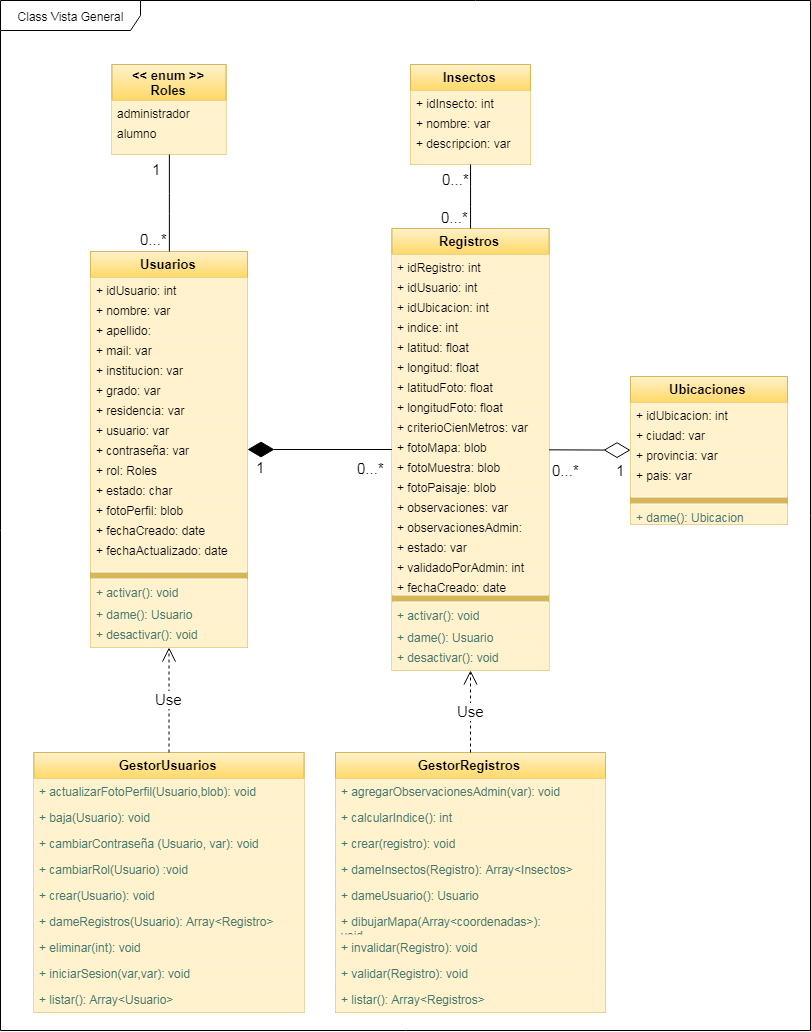
\includegraphics[width=1\textwidth]{imagenes/DiagramasUML/clase.png}
							%%Me parece que queda mejor sin el hfill
							%\hfill
					\label{fig:diagrama-clases-disenio}
			\end{figure}
	%#############################################################################
	%#   
	%#   DIAGRAMAS DE ACTIVIDAD
	%#
	%#############################################################################
	\section{Diagramas de Actividad}
		\subsection{Inicio de Sesión}
			\begin{figure}[H]
			\centering
				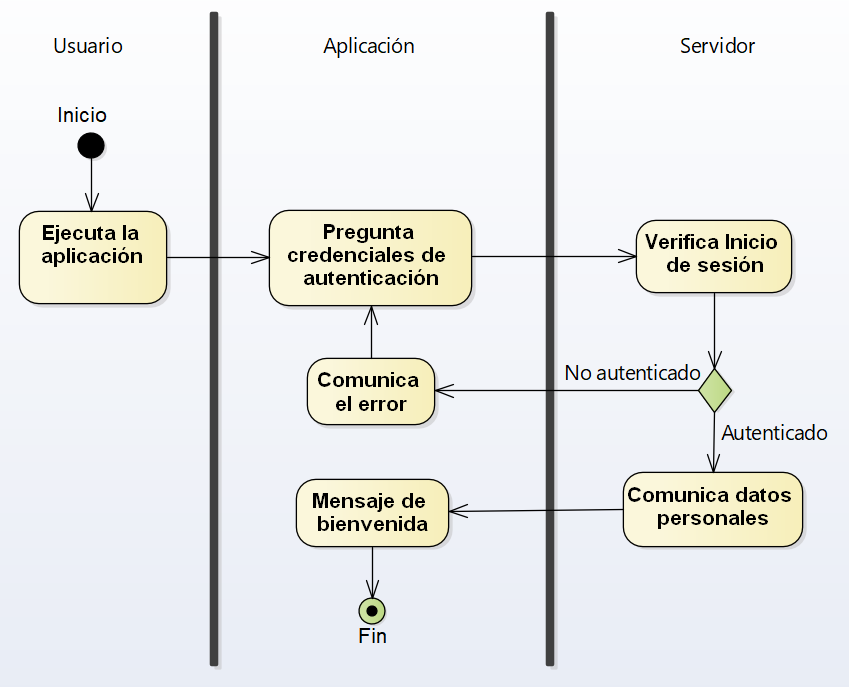
\includegraphics[width=1\textwidth]{imagenes/analisis/diagrama-actividad-inicioSesion.png}
					%%Me parece que queda mejor sin el hfill 
					%\hfill
				\label{fig:diagrama-actividad-autenticar}
			\end{figure}

		\subsection{Registrar Usuario}
			\begin{figure}[H]
			\centering
				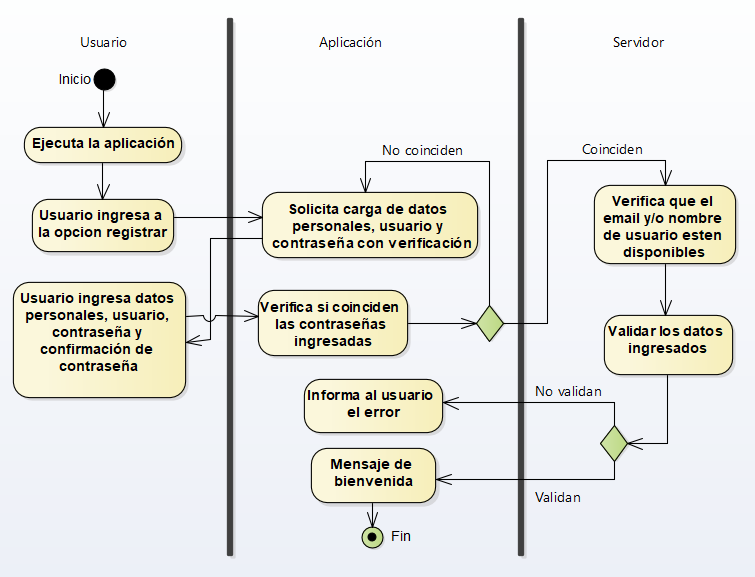
\includegraphics[width=1\textwidth]{imagenes/analisis/diagrama-actividad-registrar.png}
					%%Me parece que queda mejor sin el hfill
					%\hfill 
				\label{fig:diagrama-actividad-registrar}
			\end{figure}

		\subsection{Crear Registro }
			\begin{figure}[H]
			\centering
				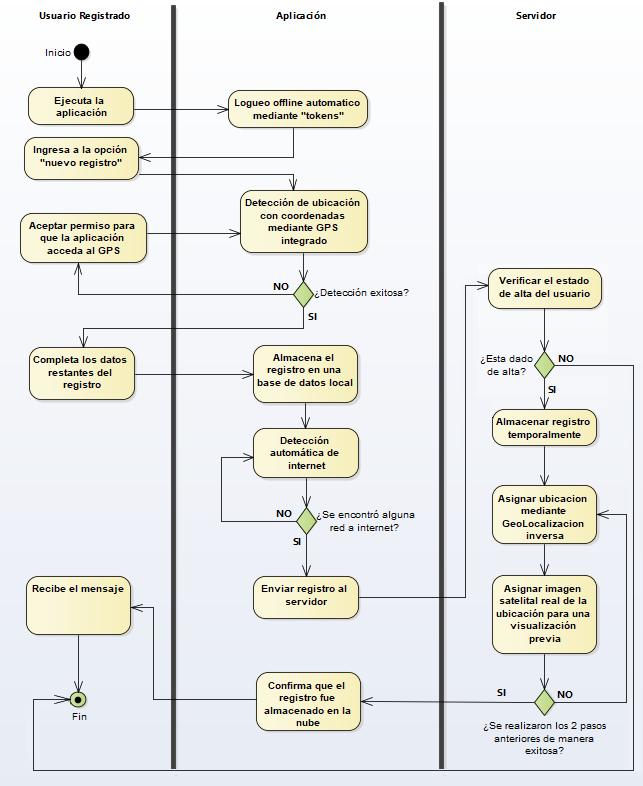
\includegraphics{imagenes/analisis/diagrama-actividad-crear-registro.png}
					%%Me parece que queda mejor sin el hfill
					%\hfill
				\label{fig:diagrama-actividad-crear-tienda}
			\end{figure}

		\subsection{Ver Mapa Interactivo}
			\begin{figure}[H]
			\centering
				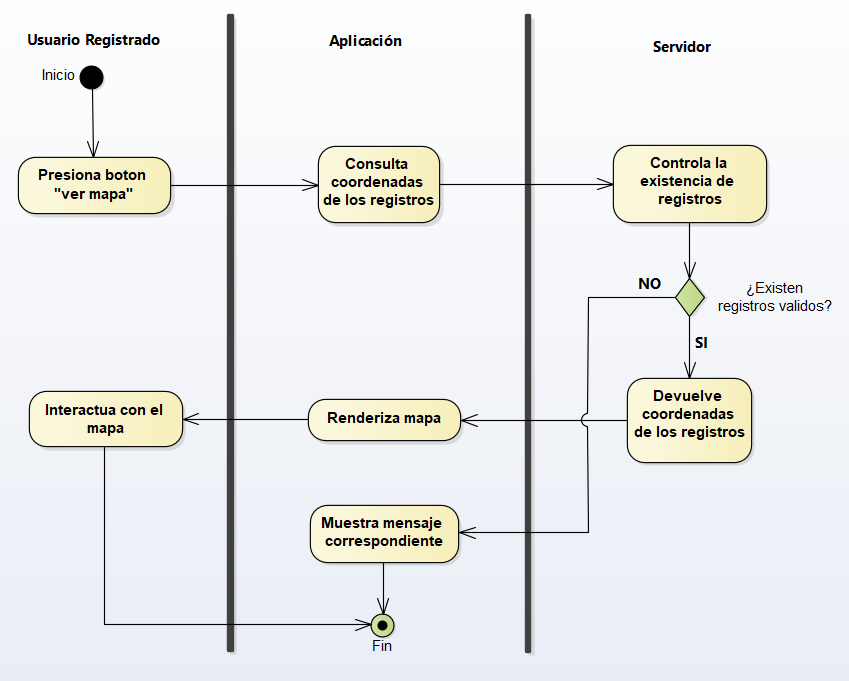
\includegraphics[width=1\textwidth]{imagenes/analisis/diagrama-actividad-ver-mapa.png}
					%%Me parece que queda mejor sin el hfill
					%\hfill
				\label{fig:diagrama-actividad-comprar-producto}
				\end{figure}
			
	%#############################################################################
	%#   
	%#   DIAGRAMAS DE SECUENCIA 
	%#
	%#############################################################################

	\section{Diagramas de Secuencia}
		\subsection{Iniciar Sesion}
			\begin{figure}[H]
				\centering
				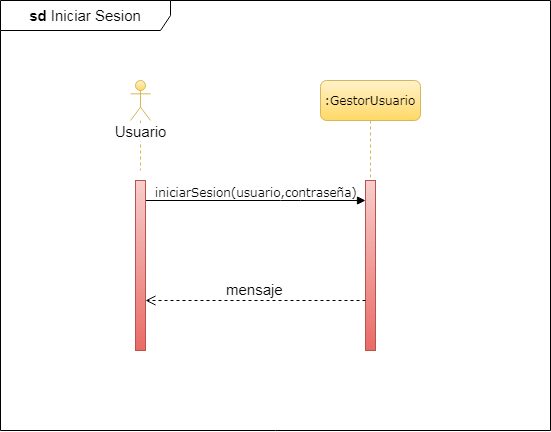
\includegraphics[width=1\textwidth]{imagenes/DiagramasUML/sdIniciarSesion.png}
							%%Me parece que queda mejor sin el hfill
							%\hfill
					\label{fig:diagrama-secuencia-autenticar}
			\end{figure}

		\subsection{Registrar}
			\begin{figure}[H]
				\centering
				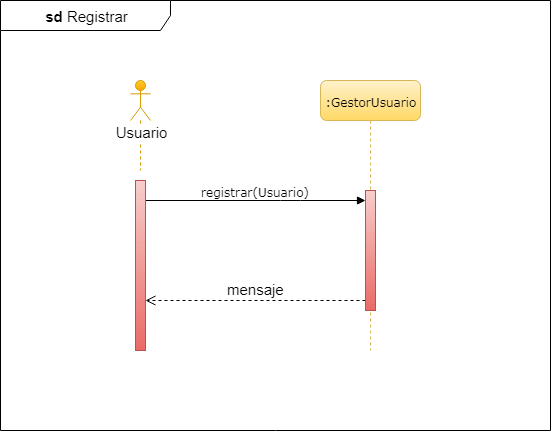
\includegraphics[width=1\textwidth]{imagenes/DiagramasUML/sdRegistrar.png}
							%%Me parece que queda mejor sin el hfill
							%\hfill
					\label{fig:diagrama-secuencia-registrar}
			\end{figure}

		\subsection{Crear Registro}
			\begin{figure}[H]
        \centering
        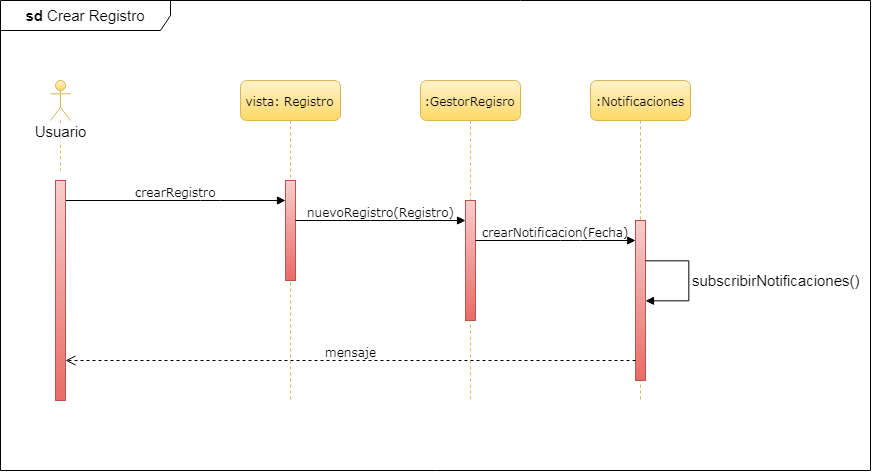
\includegraphics[width=1\textwidth]{imagenes/DiagramasUML/sdCrearRegistro.png}
							%%Me parece que queda mejor sin el hfill
							%\hfill
					\label{fig:diagrama-secuencia-crear-tienda}
			\end{figure}

	%#############################################################################
	%#   
	%#   INTERFAZ DE USUARIO
	%#
	%#############################################################################

	\section{Interfaz de usuario}
			\subsection{Aplicacion movil}

				\begin{figure}[H]
					\raggedright\textbf{Inicio de sesion}\par\medskip
					\centering
						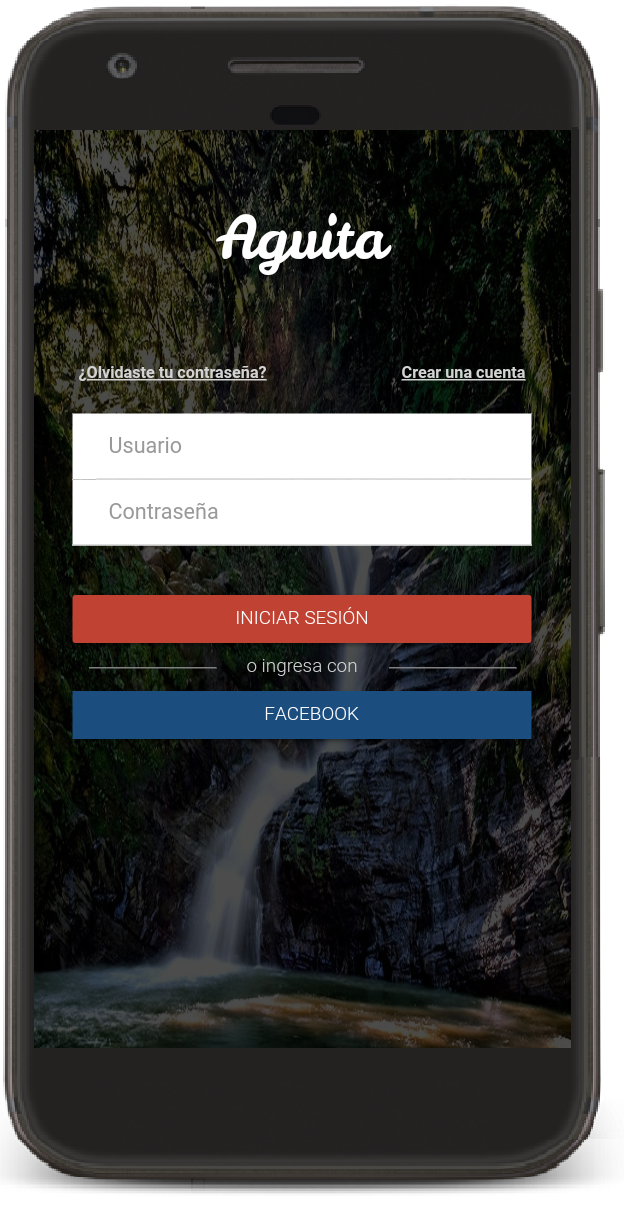
\includegraphics[width=0.6\textwidth]{Screenshots/login.png}
				\end{figure}

				\begin{figure}
					\raggedright\textbf{Configuracion}\par\medskip
					\centering
						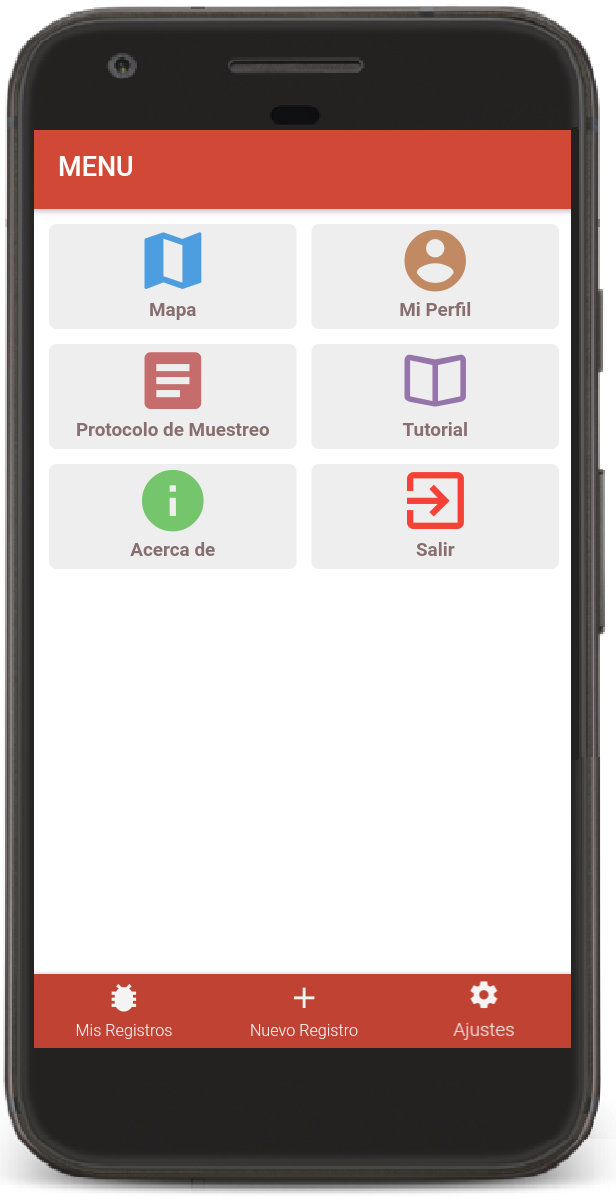
\includegraphics[width=0.6\textwidth]{Screenshots/configuracion.png}
				\end{figure}

				\begin{figure}
					\raggedright\textbf{Perfil}\par\medskip
					\centering
						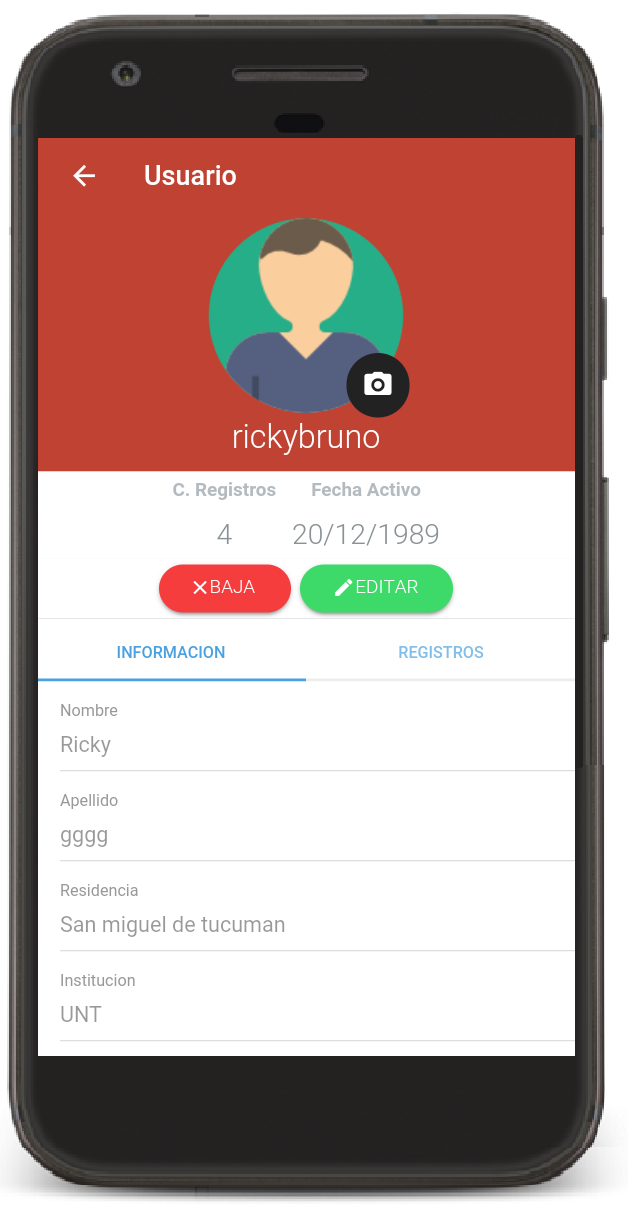
\includegraphics[width=0.6\textwidth]{Screenshots/perfil.png}
				\end{figure}

				\begin{figure}
					\raggedright\textbf{Nuevo registro}\par\medskip
					\centering
						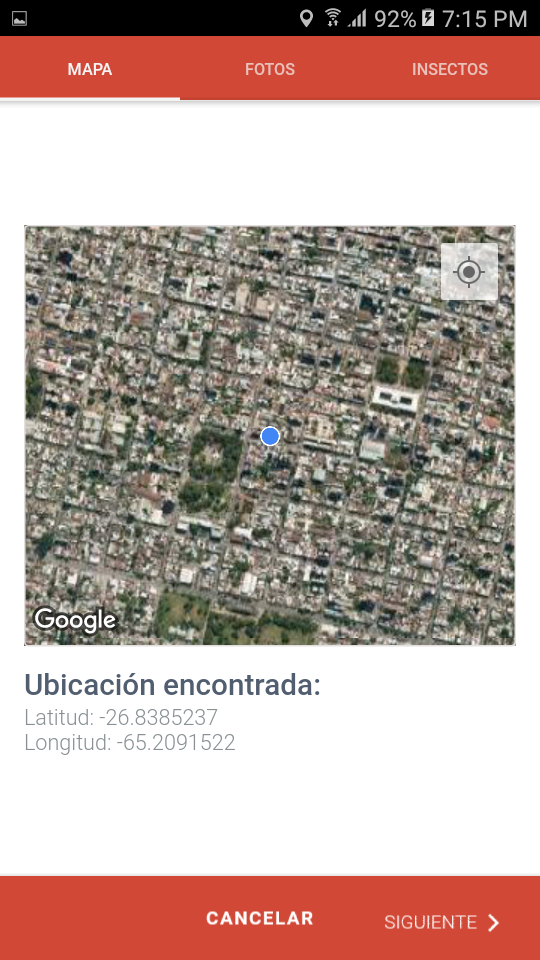
\includegraphics[width=0.6\textwidth]{Screenshots/registroPaso1.png}
						\caption{Paso 1: Obtencion automatica de coordenadas}
				\end{figure}

				\begin{figure}
					\centering
						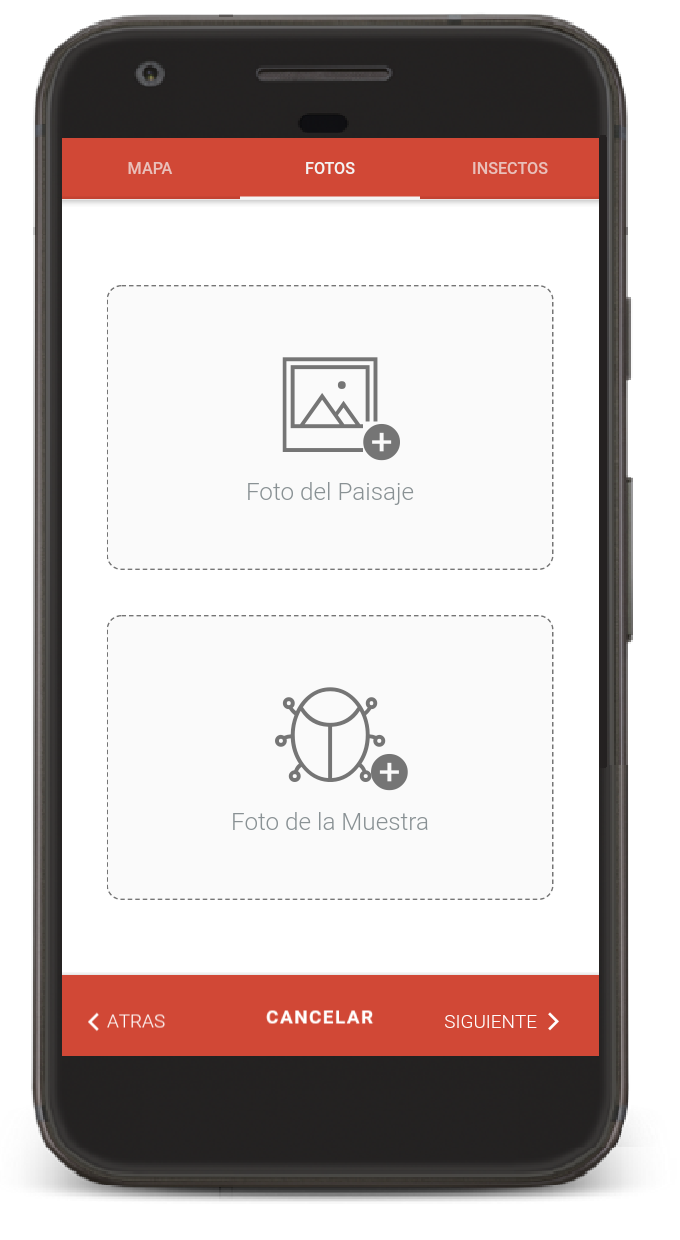
\includegraphics[width=0.6\textwidth]{Screenshots/registroPaso2A.png}
						\caption{Paso 2: Obtencion manual de fotografias (vista limpia)}
				\end{figure}

				\begin{figure}
					\centering
						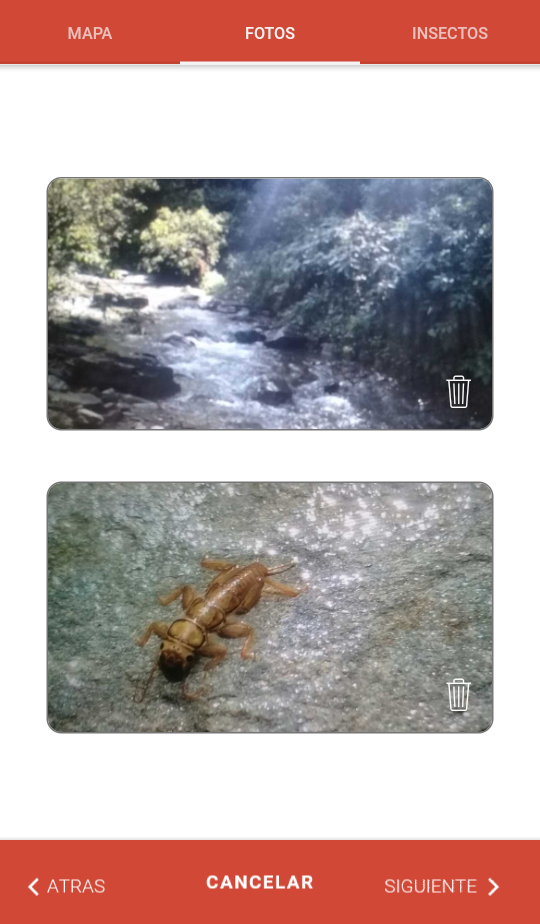
\includegraphics[width=0.6\textwidth]{Screenshots/registroPaso2B.png}
						\caption{Paso 2: Vista con fotos capturadas}
				\end{figure}
								
				\begin{figure}
					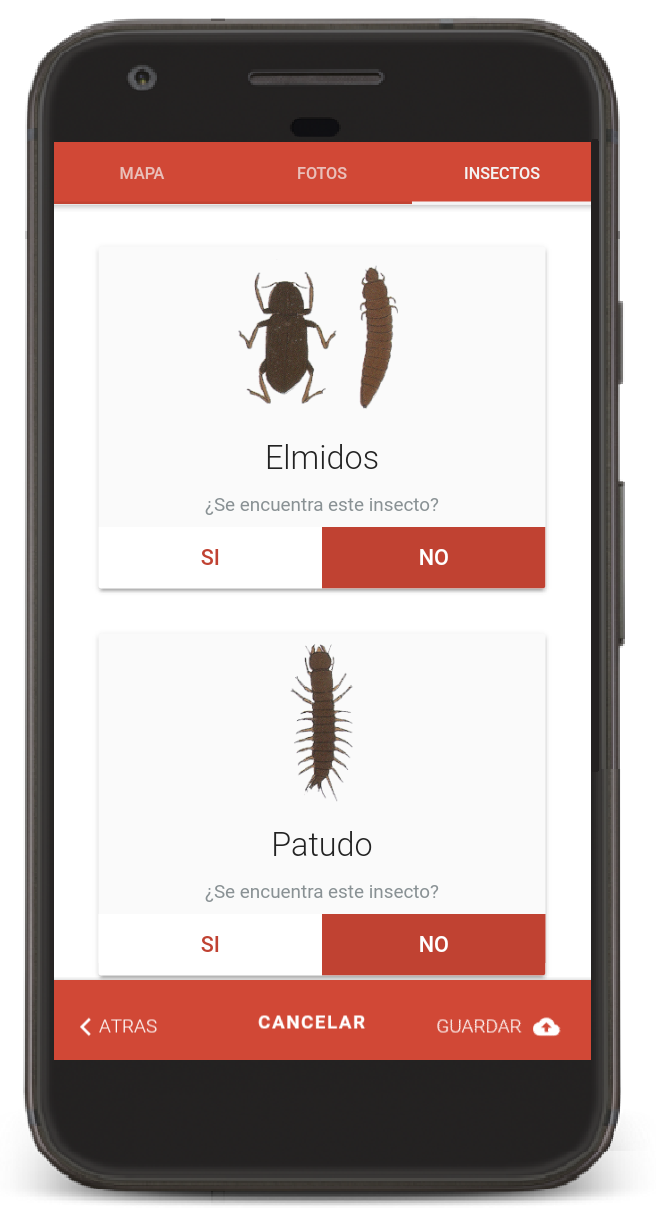
\includegraphics[width=0.3\textwidth]{Screenshots/registroPaso3A.png}
					\caption{Paso 3: Formulario con desplazamiento vertical. Screenshot 1/3}
				\end{figure}

				\begin{figure}
					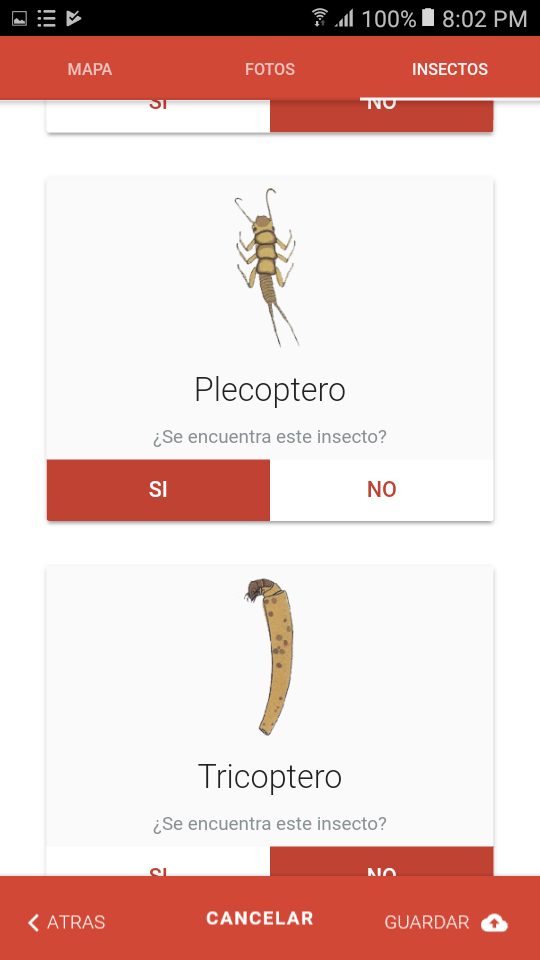
\includegraphics[width=0.3\textwidth]{Screenshots/registroPaso3B.png}
					\caption{Paso 3: Formulario con desplazamiento vertical. Screenshot 2/3}
				\end{figure}

				\begin{figure}
					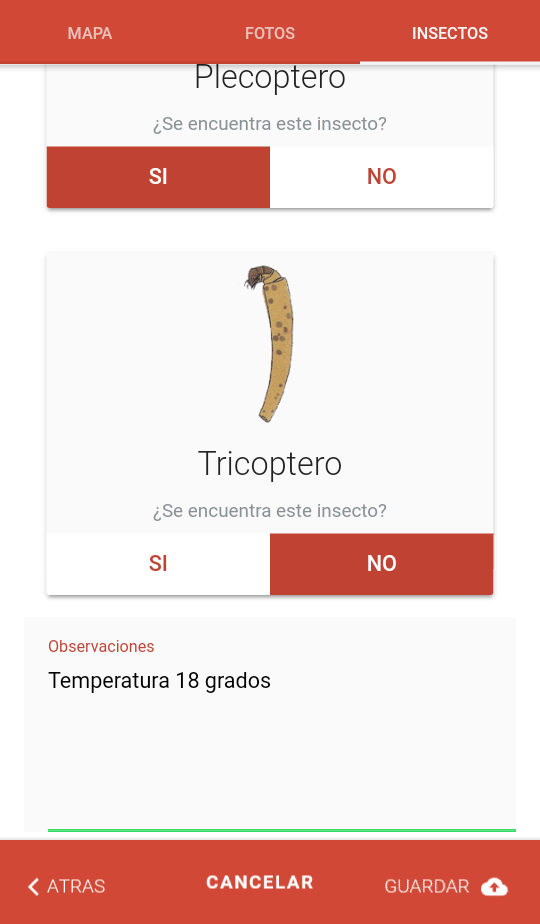
\includegraphics[width=0.3\textwidth]{Screenshots/registroPaso3C.png}
					\caption{Paso 3: Formulario con desplazamiento vertical. Screenshot 3/3}
				\end{figure}

				\begin{figure}
					\centering
						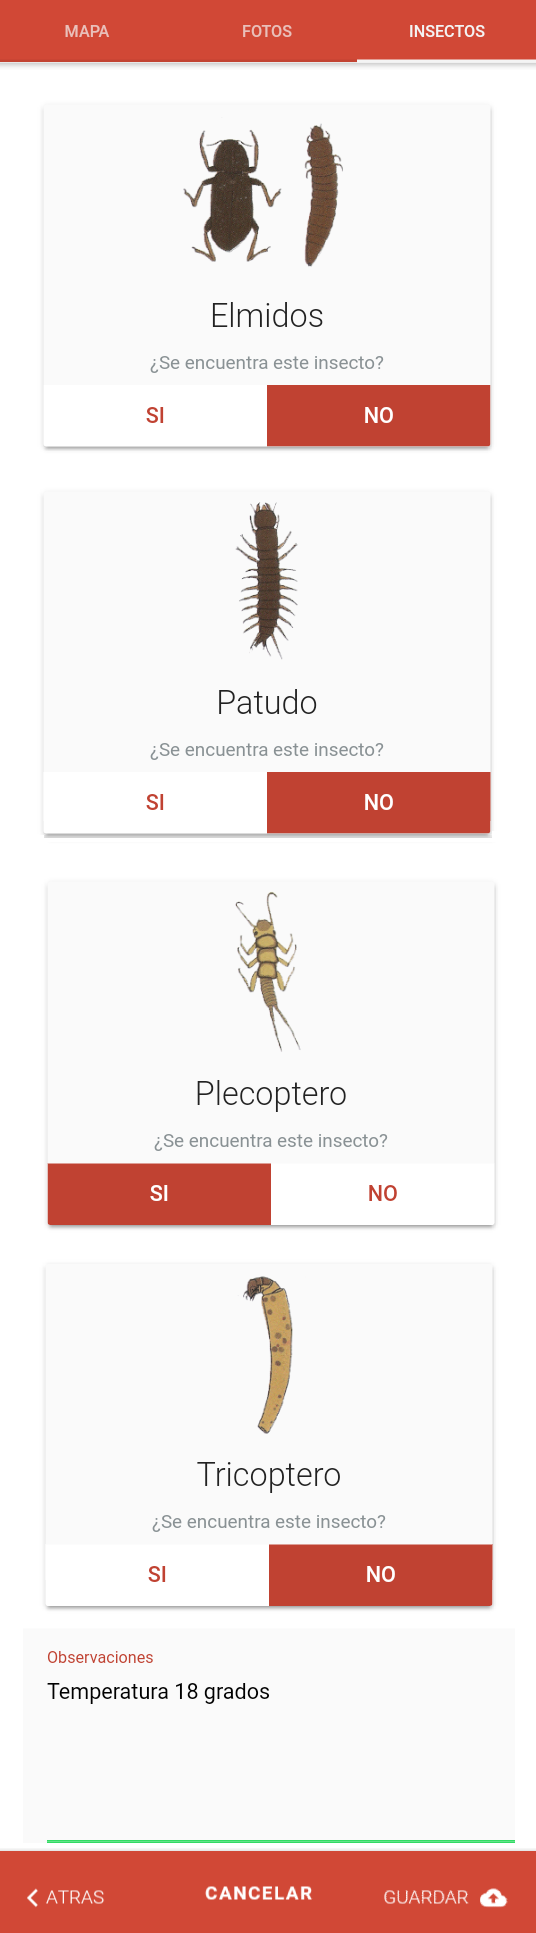
\includegraphics[height=1.5\textwidth]{Screenshots/registroPaso3Completo.png}
						\caption{Paso 3: Formulario con desplazamiento vertical. Vista completa a modo ilustrativo}
				\end{figure}

				\begin{figure}
					\centering
						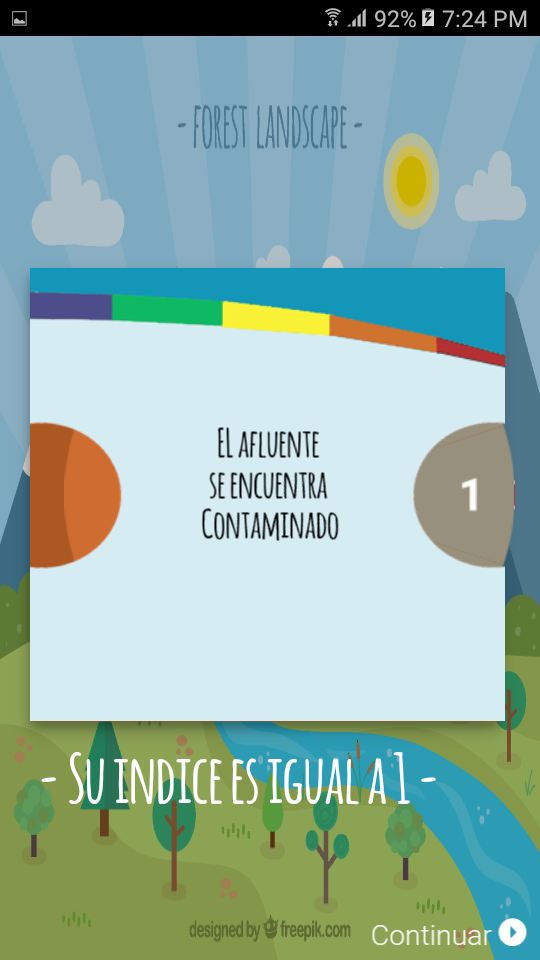
\includegraphics[width=0.6\textwidth]{Screenshots/ruedita.png}
						\caption{Paso 4: Ruleta animada indicadora de indice segun coincidencias de insectos}
				\end{figure}

				\begin{figure}
					\raggedright\textbf{Listar registros creados}\par\medskip
					\centering
						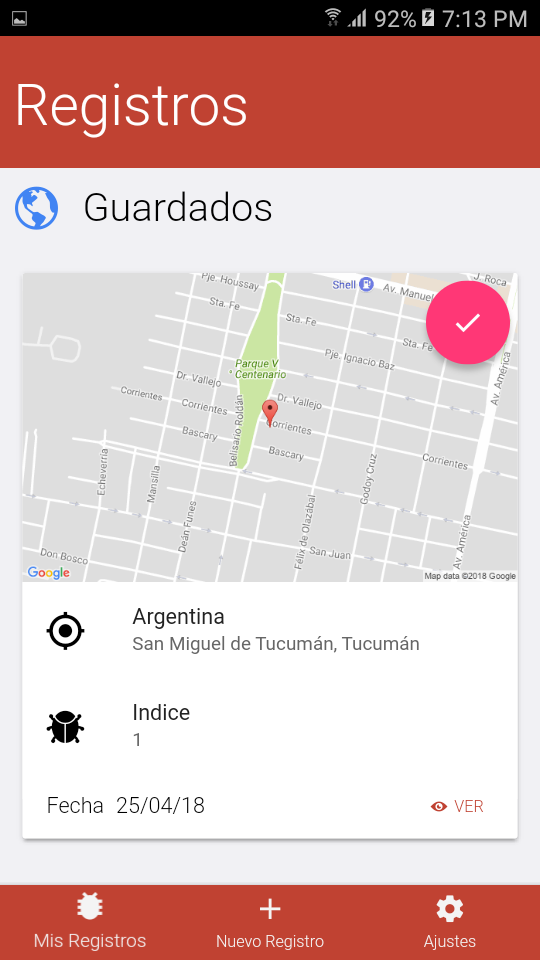
\includegraphics[width=0.6\textwidth]{Screenshots/registrosLocales.png}
						\caption{Lista con desplazamiento vertical para ver registros correspondientes al usuario logueado}
				\end{figure}

				\begin{figure}
					\raggedright\textbf{Ver registro}\par\medskip
					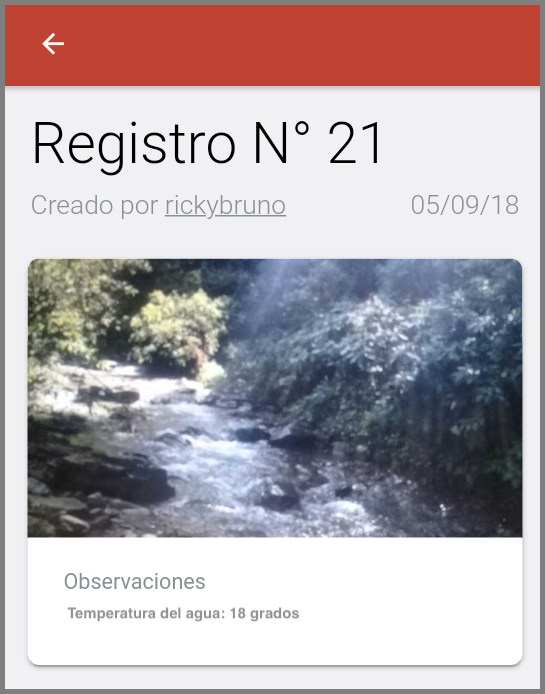
\includegraphics[width=0.3\textwidth]{Screenshots/verRegistro1.png}
					\caption{Vista de registro creado. Imagen 1/3}
				\end{figure}
				
				\begin{figure}
					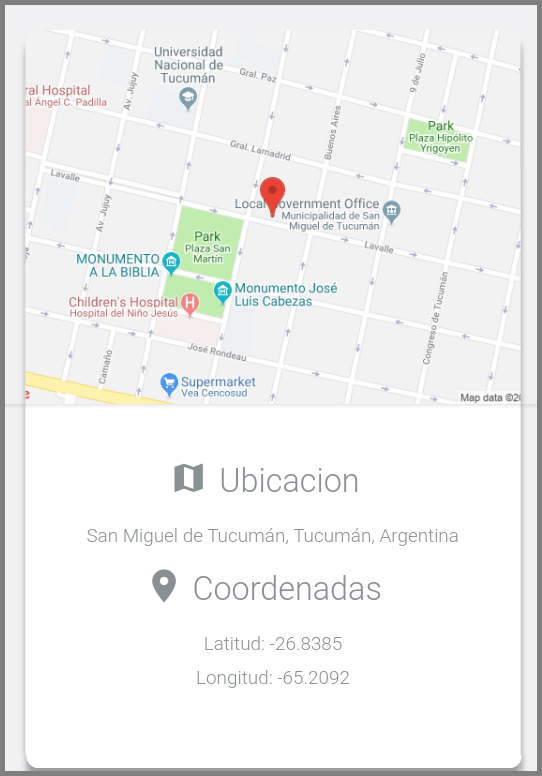
\includegraphics[width=0.3\textwidth]{Screenshots/verRegistro2.png}
					\caption{Vista de registro creado. Imagen 2/3}
				\end{figure}
				
				\begin{figure}
					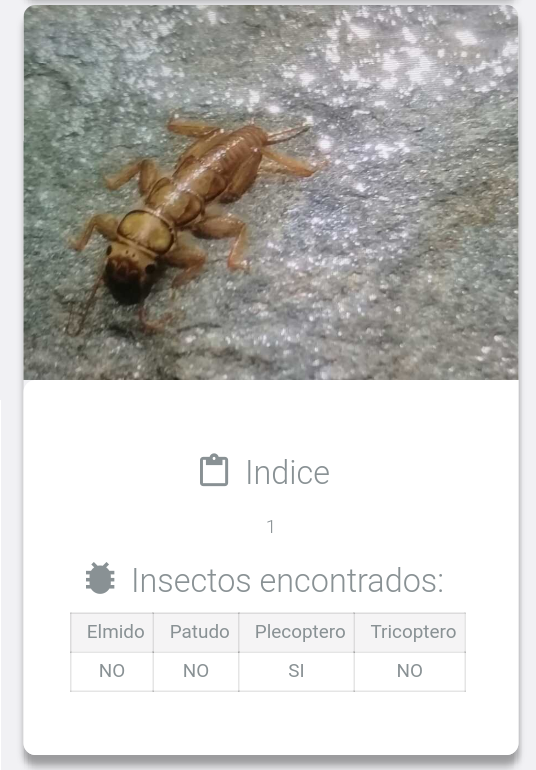
\includegraphics[width=0.3\textwidth]{Screenshots/verRegistro3.png}
					\caption{Vista de registro creado. Imagen 3/3}
				\end{figure}

				\begin{figure}
					\centering
						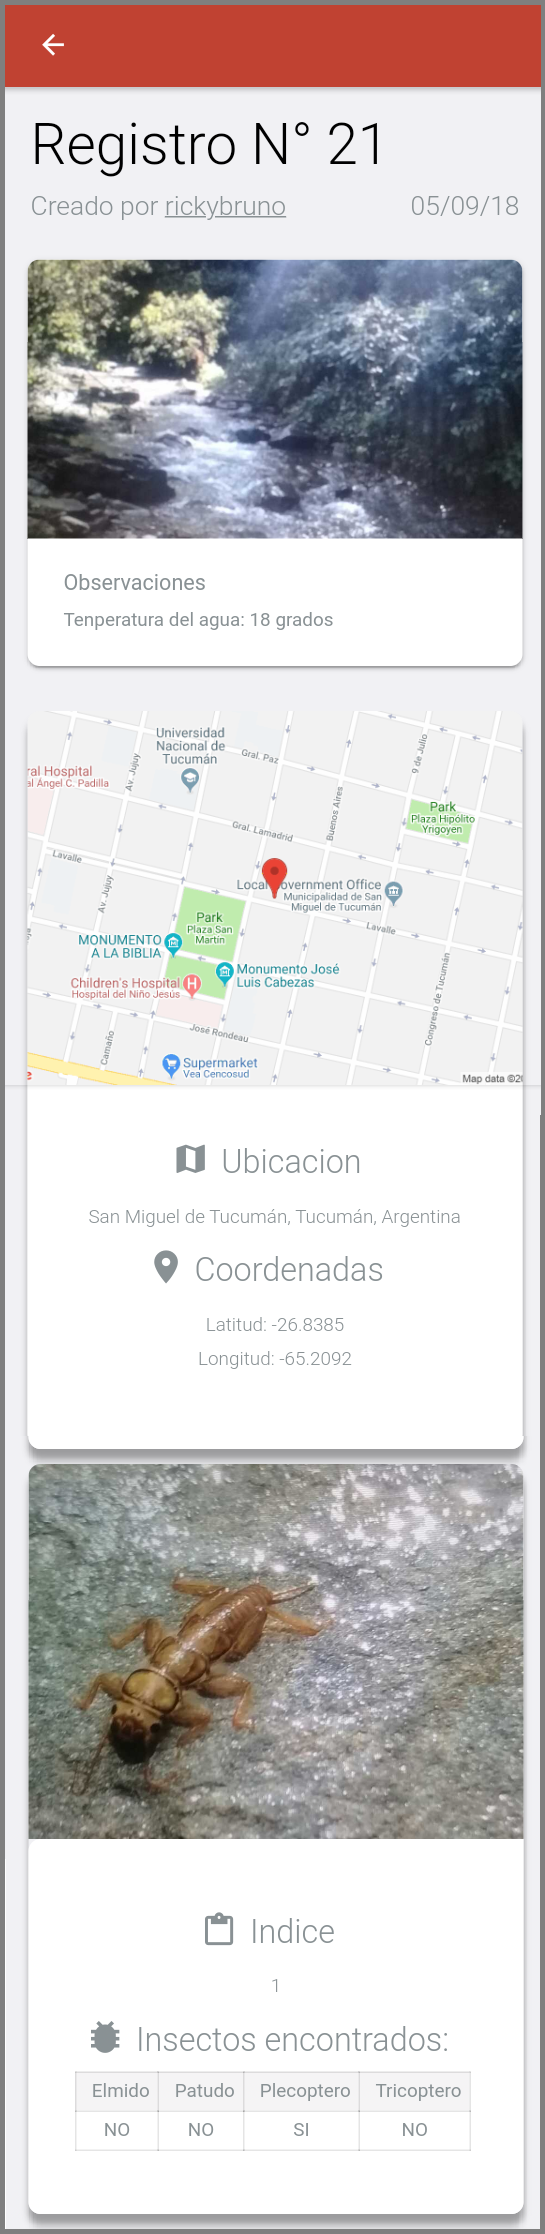
\includegraphics[height=1.5\textwidth]{Screenshots/verRegistroCompleto.png}
						\caption{Vista completa de un registro con desplazamiento vertical. Modo ilustrativo}
				\end{figure}

			\subsection{Sistema de gestion WEB}
				\begin{figure}
					\centering
						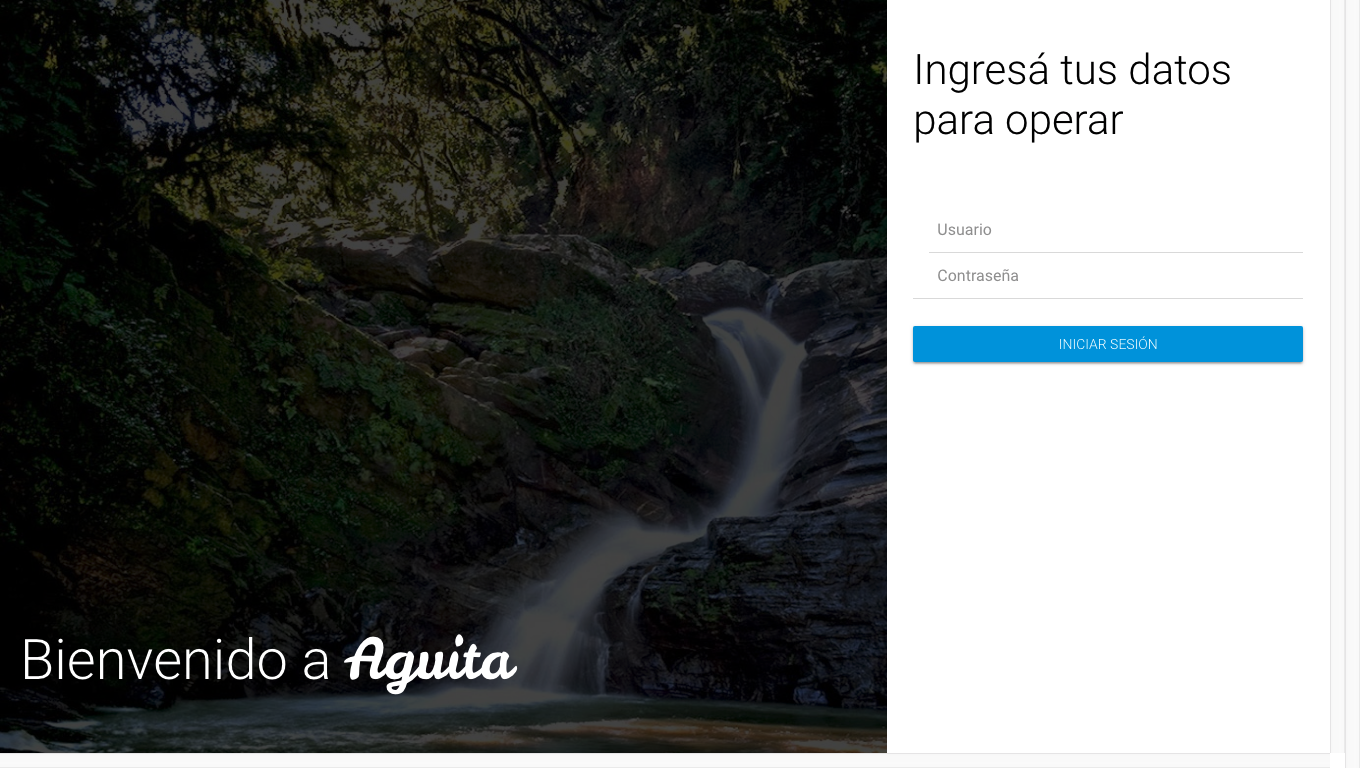
\includegraphics[width=0.6\textwidth]{Screenshots/web/login.png}
								%%Me parece que queda mejor sin el hfill
								%\hfill

				\end{figure}

	
				\begin{figure}
					\centering
						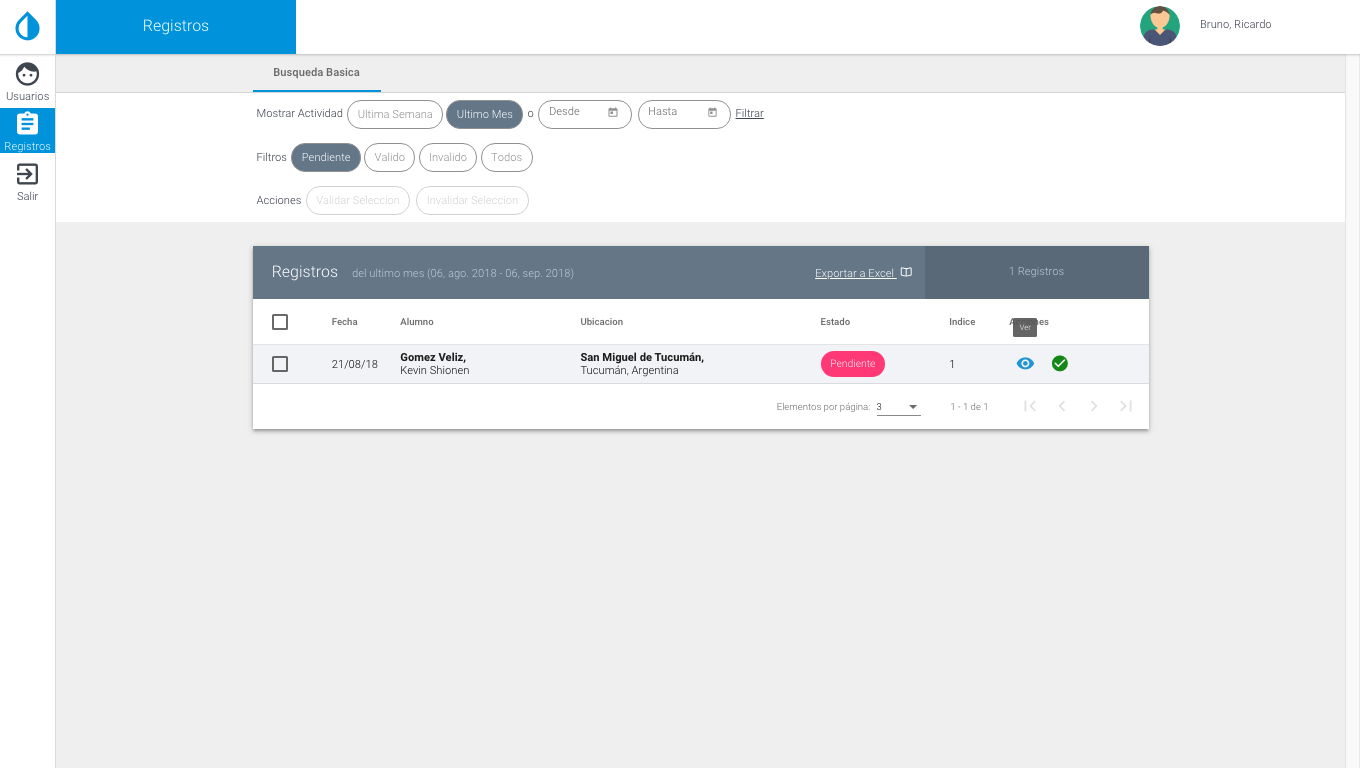
\includegraphics[width=0.6\textwidth]{Screenshots/web/registroListar.png}
								%%Me parece que queda mejor sin el hfill
								%\hfill
								\caption{Pantalla de resultados de la busqueda de registros con filtros}
						\label{fig:busqueda}
				\end{figure}

			
				\begin{figure}
					\centering
						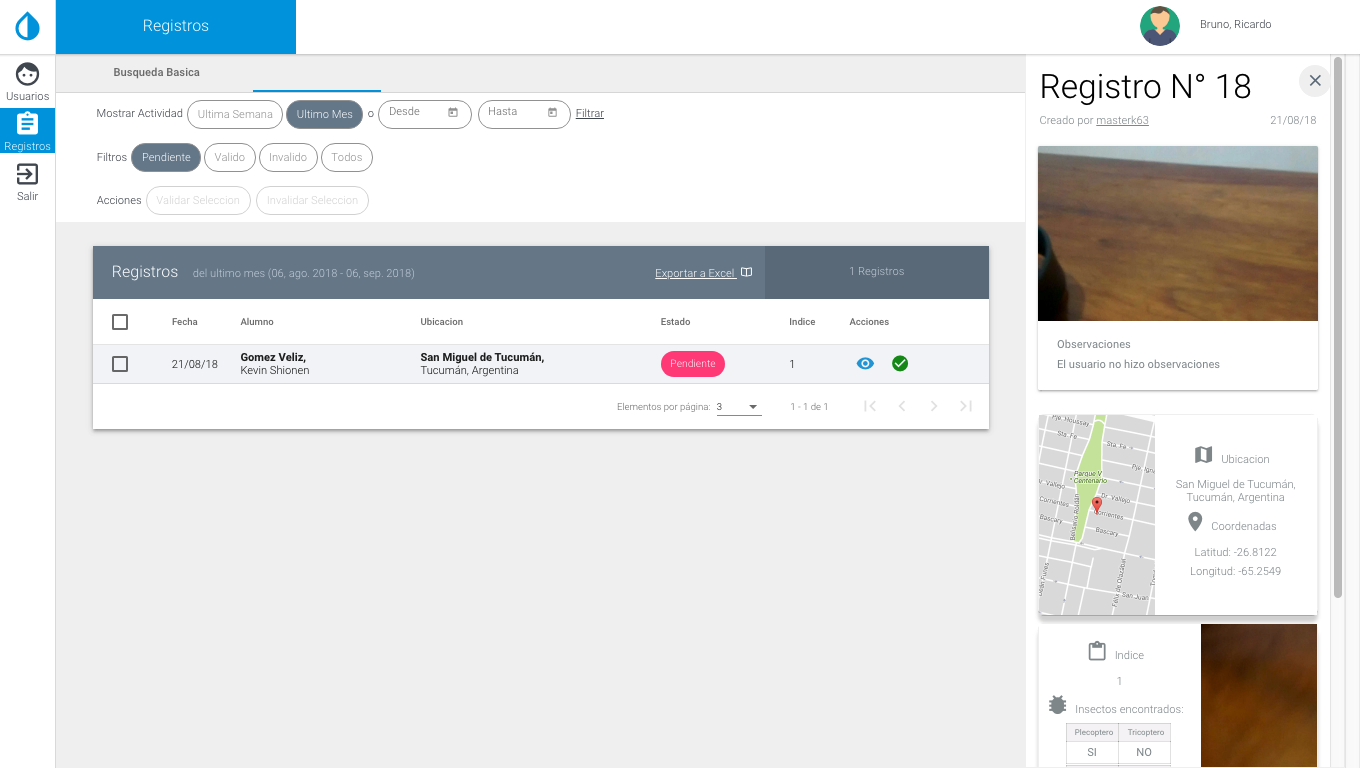
\includegraphics[width=0.6\textwidth]{Screenshots/web/registroVer1.png}
								%%Me parece que queda mejor sin el hfill
								%\hfill
								\caption{Visualizacion rapida de registro en el sector derecho de la pantalla}
				\end{figure}

				\begin{figure}
					\centering
						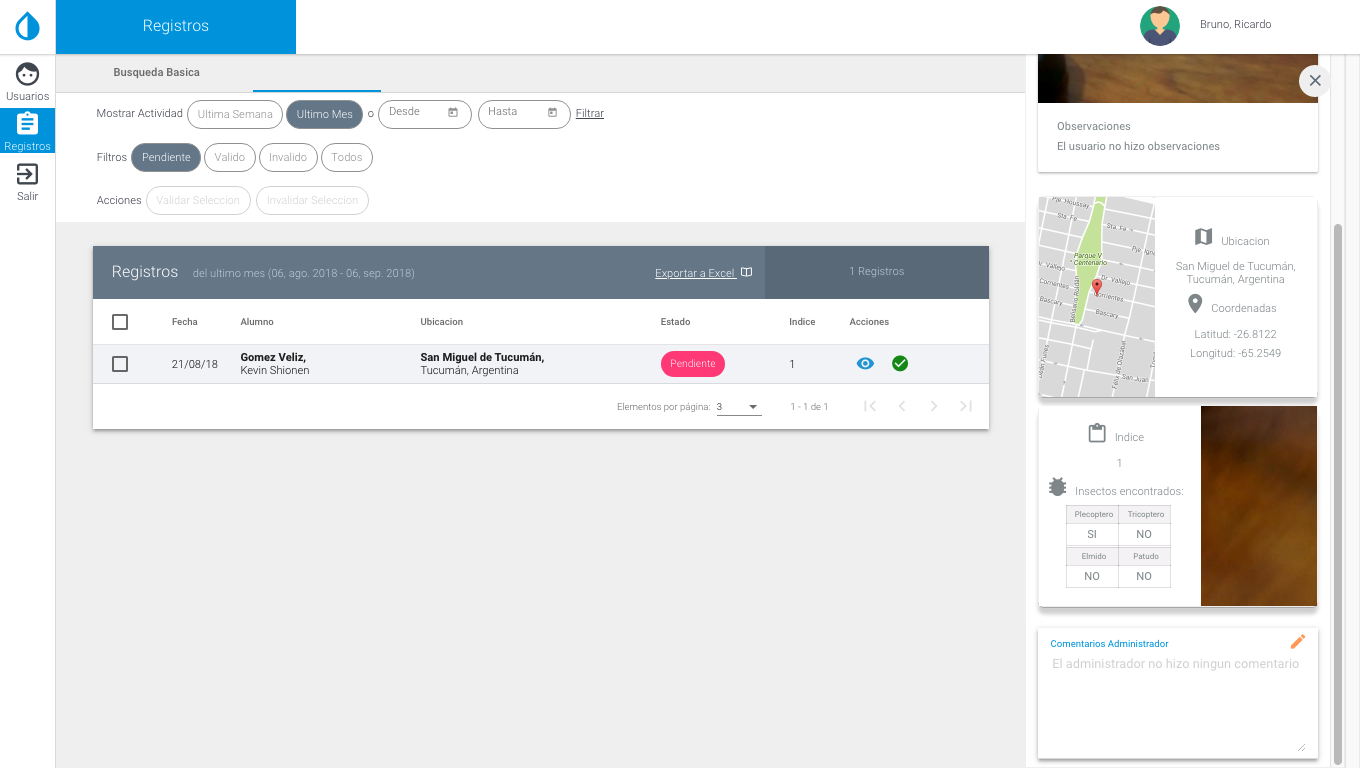
\includegraphics[width=0.6\textwidth]{Screenshots/web/registroVer2.png}
								%%Me parece que queda mejor sin el hfill
								%\hfill
								\caption{Visualizacion rapida de registro en el sector derecho de la pantalla}

				\end{figure}

			
				\begin{figure}
					\centering
						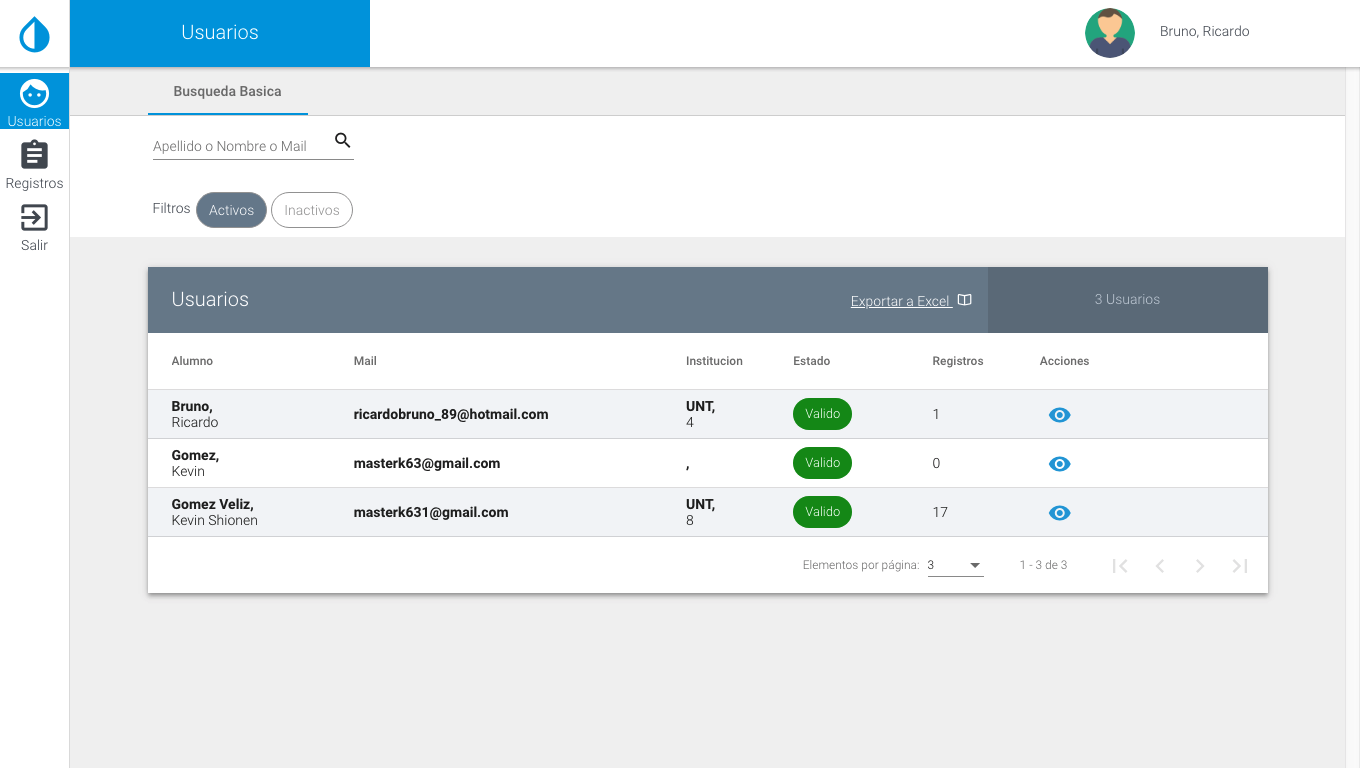
\includegraphics[width=0.6\textwidth]{Screenshots/web/usuarioListar.png}
								%%Me parece que queda mejor sin el hfill
								%\hfill
								\caption{Pantalla de resultados de la busqueda de usuarios con filtros}
						
				\end{figure}

			
				\begin{figure}
					\centering
						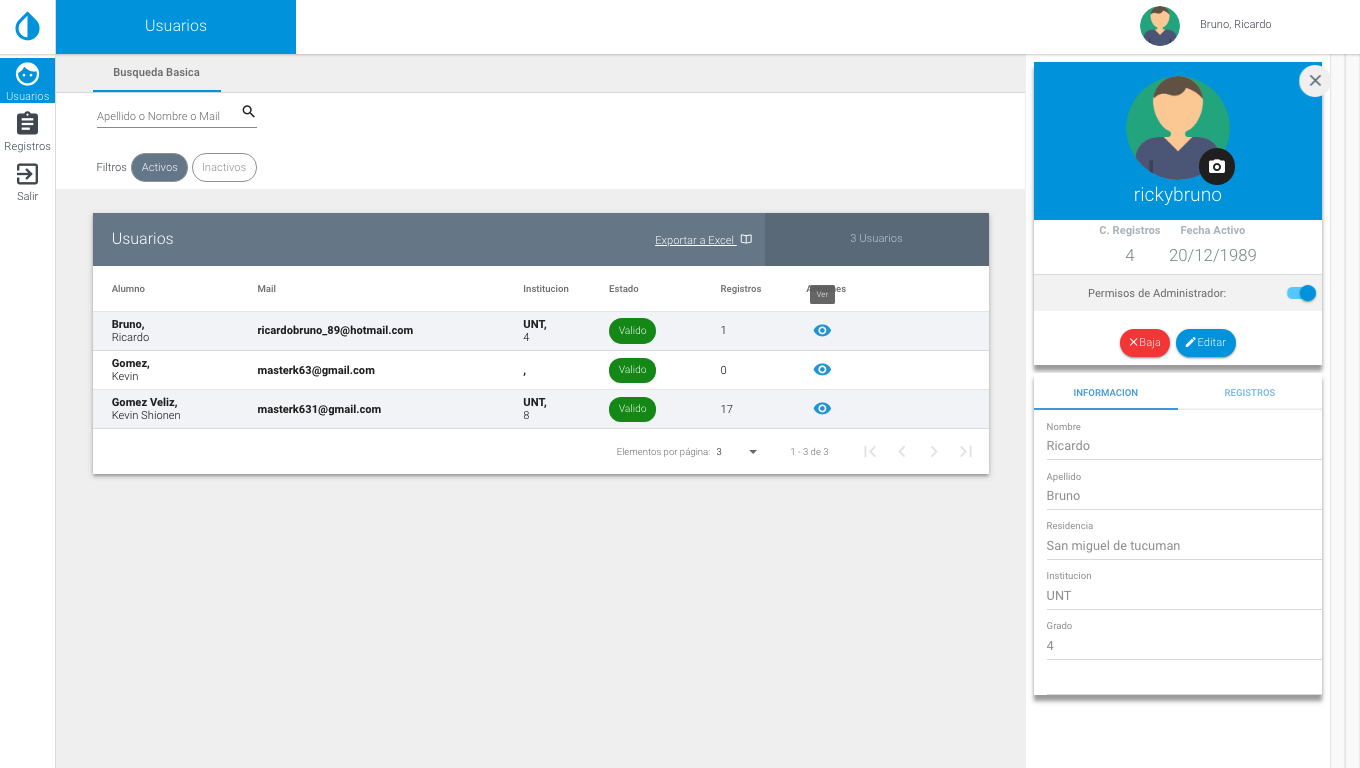
\includegraphics[width=0.6\textwidth]{Screenshots/web/usuarioVer.png}
								%%Me parece que queda mejor sin el hfill
								%\hfill
								\caption{Visualizacion rapida del perfil de usuario en el sector derecho de la pantalla}

				\end{figure}
